
%----------------------------------------------------------------------------------------
%	PART
%----------------------------------------------------------------------------------------


\part{Capítulo cuatro}

\graphicspath{ {4_Capitulo/img/ejemplos/},{4_Capitulo/img/explicacion/}, {W_Varios/2_Portada_capitulos} }
\definecolor{MyOrange}{RGB}{255,177,131}
%----------------------------------------------------------------------------------------
%	CHAPTER 4
%----------------------------------------------------------------------------------------

\chapterimage{4_Capitulo/img/portada/ima2.jpg} % Chapter heading image


\chapter{Serie uniforme vencida y anticipada}

\begin{figure}[H]
    \centering
    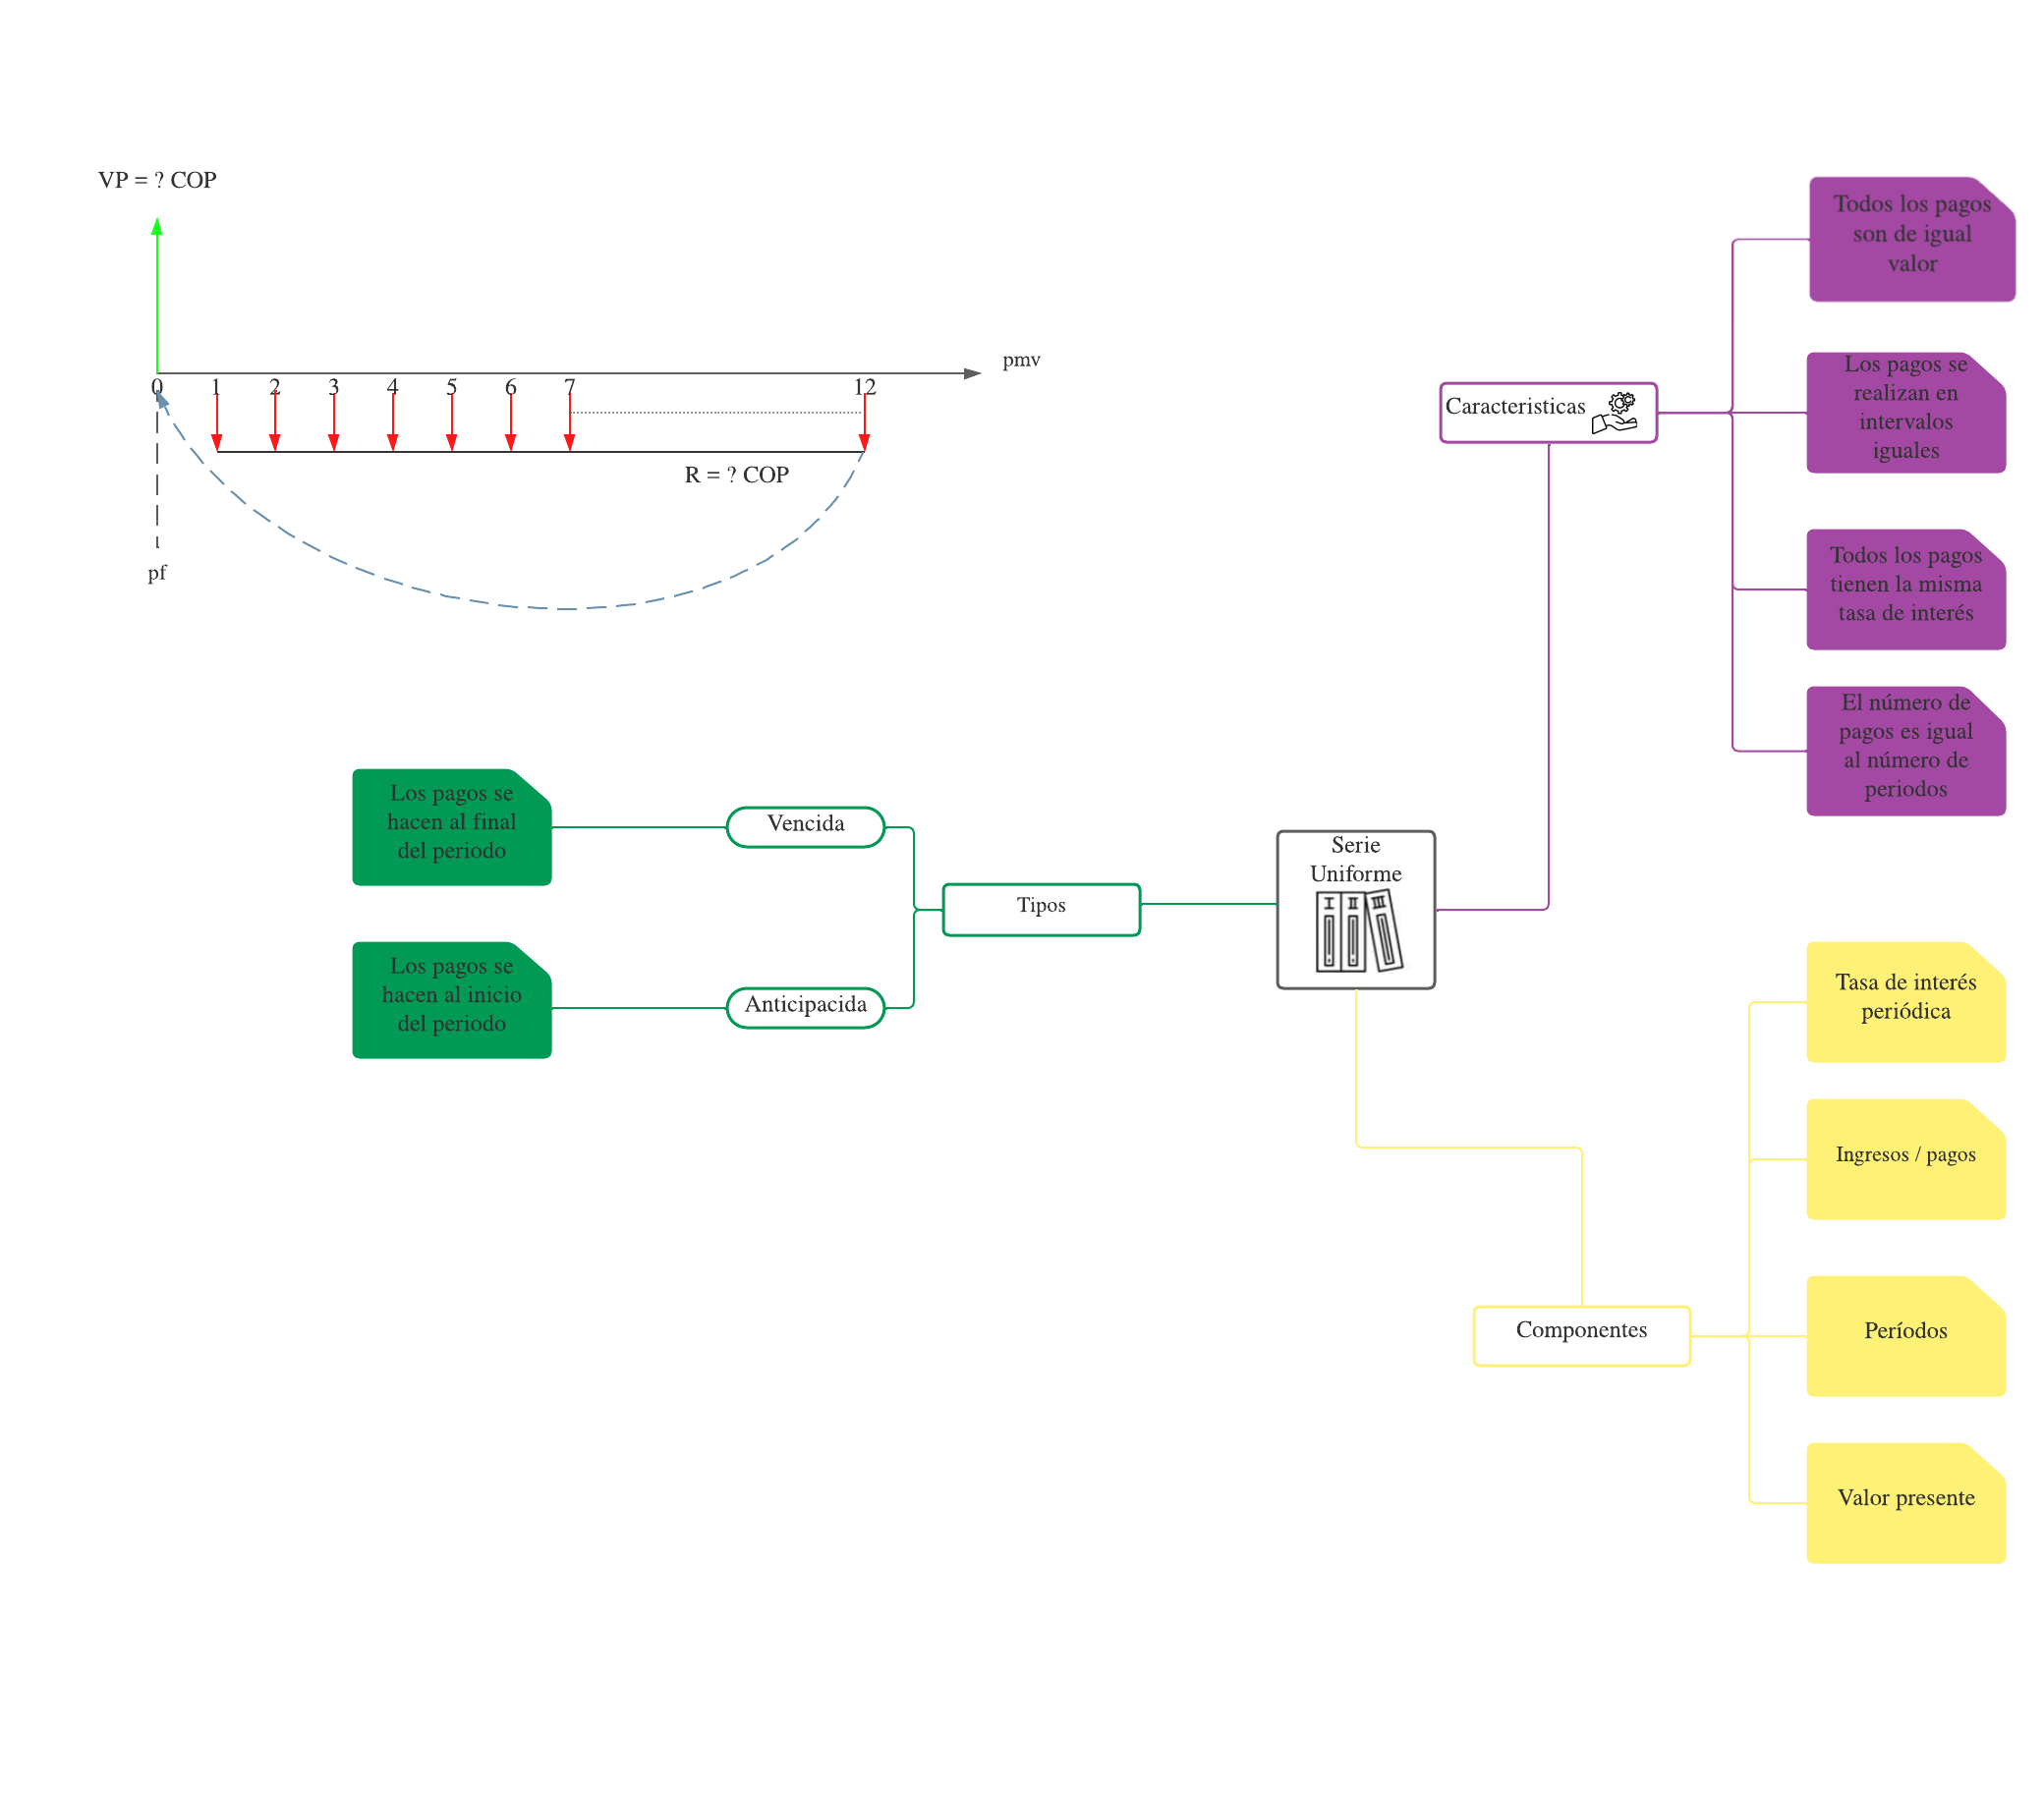
\includegraphics[scale=0.3]{4_Capitulo/img/ejemplos/Exportados/Mapa mental .png}
\end{figure}

\newpage

\section{{Fórmulas del capítulo}}

\begin{spacing}{1.2}
	\begin{center}
		\begin{tabular}{ |p{4.2cm}|p{5.7cm}| p{4cm}|}
			\hline
			\rowcolor{MyOrange}              %
			\begin{center}\textbf{Fórmula} \end{center}                                      & \begin{center} \textbf{Nombre}\end{center}                         & \begin{center} \textbf{Excel} \end{center} \\ \hline


			$VP = R  \frac{1-(1 + i)^{-n}}{i} $\hspace{35pt}               & Valor presente serie uniforme vencida             & VNA(i;R1;R2;R3;...)       \\ \hline


			$VF = R  \frac{(1 + i)^n-1}{i} $                               & Valor futuro serie uniforme vencida \hspace{35pt} & VF(i;n;;VA,0)             \\  \hline


			$VP_{a} = R  \frac{1-(1 + i)^{-n}}{i}  (1 + i) $ \hspace{35pt} & Valor presente serie uniforme anticipada          & -                         \\ \hline

			$VF_{a} = R  \frac{(1 + i)^n-1}{i}   (1 + i) $ \hspace{35pt}   & Valor futuro serie uniforme anticipada            & VF(i;n;;VA,1)             \\ \hline
		\end{tabular}
	\end{center}
\end{spacing}

%%%%%%%%%% NO OLVIDAR COLOCAR ESTE COMENTARIO CON EL NUMERO DE EJERCICIO %%%%%%%%%%%%%
%%%%%%%%%%%%%%%%%%% EJERCICIO 1 %%%%%%

%%%%%%%%%% NO OLVIDAR COLOCAR ESTE COMENTARIO CON EL NUMERO DE EJERCICIO %%%%%%%%%%%%%
%%%%%%%%%%%%%%%%%%% EJERCICIO 1 %%%%%%
%%Text bf para negrilla , el \\ es para el salto de linea.
%%El primer \\ hace un espacio en el texto y el 2 \\ crea otro espacio

\textbf{Ejemplo 1}\newline
Una persona compra un terreno cuyo valor al contado es de 2.000.000 COP. Si le dan la facilidad para pagarlo en cuatro periodos trimestre vencidos del mismo valor cada uno y, además se le cargará un interés del 40\% nominal anual trimestre vencido, hallar el valor de la cuota trimestral de amortización.\\ \\

\textbf{Solución.}\\
\begin{center}

	\renewcommand{\arraystretch}{1.5}% Margenes de las celdas
	%Creación de la cuadricula
	\begin{longtable}{|C{0.3\linewidth}|C{0.3\linewidth}|C{0.3\linewidth}| }
		%Creamos una linea horizontal
		\hline
		%Definimos el color de la primera fila
		\rowcolor[HTML]{FFB183}
		%%%%% INICIO ASIGNACIÓN FECHA FOCAL %%%%%%%
		%%%%%%%%%% INICIO TITULO
		%Lo que se hace aquí es mezclar las 3 columnas en una sola
		\multicolumn{3}{|c|}{\cellcolor[HTML]{FFB183}\textbf{1. Asignación período focal}}   \\ \hline
		%%%%%%%%%% FIN TITULO
		%%%%% INICIO DECLARACIÓN DE VARIABLES %%%%%%%
		\multicolumn{3}{|c|}{$pf : 0 ptv$} \\ \hline
		%Definimos el color de la primera fila
		\rowcolor[HTML]{FFB183}
		%%%%% INICIO DECLARACIÓN DE VARIABLES %%%%%%%
		%%%%%%%%%% INICIO TITULO
		\multicolumn{3}{|c|}{\cellcolor[HTML]{FFB183}\textbf{2. Declaración de variables}}                                                                                   \\ \hline
		%%%%%%%%%% FIN TITULO
		%%%%%%%%%% INICIO DE MATEMÁTICAS
		\multicolumn{1}{|c|}{\cellcolor[HTML]{FFB183}\textbf{Valores monetarios}}    & \multicolumn{1}{c|}{\cellcolor[HTML]{FFB183}\textbf{Valores no monetarios}} & \multicolumn{1}{c|}{\cellcolor[HTML]{FFB183}\textbf{Incógnitas}} \\ \hline
		VP = 2.000.000 COP & $j_ {1} = 40\% \textit{ natv} \equiv 10\% \textit{ptv} = i_1$ & $ R = { ? } COP $ \\
		& $n_{1}= 1 \textit{ ptv}$ & \\
		& $n_{2}= 2 \textit{ ptv}$ & \\
		& $n_{3}= 3 \textit{ ptv}$ & \\
		& $n_{4}= 4 \textit{ ptv}$ & \\ \hline
		%%%%%%%%%% FIN DE MATEMÁTICAS
		%%%%% FIN DECLARACIÓN DE VARIABLES


		%%%%% INICIO FLUJO DE CAJA
		\rowcolor[HTML]{FFB183}
		\multicolumn{3}{|c|}{\cellcolor[HTML]{FFB183}\textbf{3. Diagrama de flujo de caja}}                                                                                  \\ \hline
		%Mezclamos 3 columnas y pondremos el dibujo
		%%%%%%%%%%%%% INSERCIÓN DE LA IMAGEN
		\multicolumn{3}{|c|}{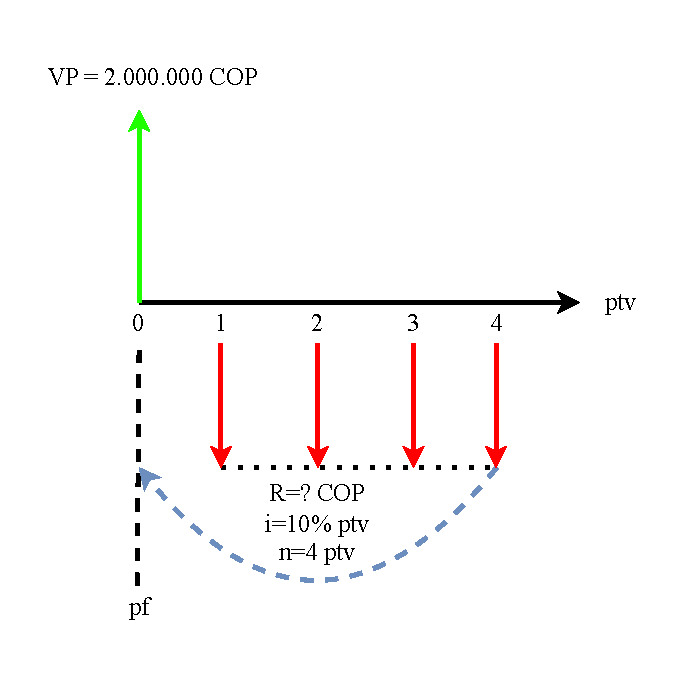
\includegraphics[trim=-5 -5 -5 -5, scale=0.8]{4_Capitulo/img/ejemplos/1/Exportados/Graficas Latex - Ejemplo 1.pdf} }                                   \\ \hline
		%%%%%%%%%%%%% FIN INSERCIÓN DE IMAGEN

		%%%%%FIN FLUJO DE CAJA



		%%%%% INICIO DECLARACIÓN FORMULAS
		%%%%%%%%%%% INICIO TITULO
		\rowcolor[HTML]{FFB183}
		\multicolumn{3}{|c|}{\cellcolor[HTML]{FFB183}\textbf{4. Declaración de fórmulas}}                                                                                    \\ \hline
		%%%%%%%%%%% FIN TITULO
		%%%%%%%%%%% INICIO MATEMÁTICAS
		\multicolumn{3}{|c|} {$VP=R\frac{1-(1+i)^{-n}}{i}$ Valor presente serie uniforme vencida}   \\
		\multicolumn{3}{|c|} {$P=F(1+i)^{-n}$ Valor presente}   \\ \hline
		%%%%%%%%%% FIN MATEMÁTICAS
		%%%%%% INICIO DESARROLLO MATEMÁTICO
		\rowcolor[HTML]{FFB183}
		%%%%%%%%%%INICIO TITULO
		\multicolumn{3}{|c|}{\cellcolor[HTML]{FFB183}\textbf{5. Desarrollo matemático}}                                                                                      \\ \hline
		%%%%%%%%%% FIN TITULO
		%%%%%%%%%% INICIO MATEMÁTICAS
		%%% - DESARROLLO MEDIANTE VALOR PRESENTE -
		\multicolumn{3}{|c|}{\cellcolor[HTML]{FFB183}\textbf{Resolviendo el problema utilizando la fórmula de valor presente}}\\ \hline
		\multicolumn{3}{|c|}{ P = 2.000.000 \ $n = 1, 2, 3, 4$ \quad } \\
		\multicolumn{3}{|c|}{  2.000.000 COP =$ R(1 + 0,1)^{−1} + R(1 + 0,1)^{−2}+R(1+0,1)^{−3} + R(1+0,1)^{−4}$}\\
		\multicolumn{3}{|c|}{  2.000.000 COP =$ R[(1+0,1)^{−1} + (1+0,1)^{−2} + (1+0,1)^{−3}+ (1 + 0, 1) ^{−4} ]$} \\
		\multicolumn{3}{|c|}{  2.000.000 COP =$ R(3,169865)$}\\
		\multicolumn{3}{|c|}{ R = 2.000.000 COP / 3,169865}\\
		\multicolumn{3}{|c|}{ R = 630.942 COP}\\ \hline
		%%%%%%%%%% DE FORMA RESOLVIENDO MEDIANTE VALOR PRESENTE SERIE UNIFORME
		\multicolumn{3}{|c|}{\cellcolor[HTML]{FFB183}\textbf{Resolviendo el problema utilizando la fórmula de valor presente serie uniforme}}\\ \hline
		\multicolumn{3}{|c|}{ VP = 2.000.000 \ $n =4$ \ $i =0.1 $ \quad} \\
		\multicolumn{3}{|c|}{ 2.000.000 COP= $ R\frac{1-(1+0.1)^{-4}}{0.1} $}\\
		\multicolumn{3}{|c|}{ 2.000.000 COP= $ R(3,16987) $}\\
		\multicolumn{3}{|c|}{ R= $ \frac{2.000.000 COP}{3,16987} $}\\
		\multicolumn{3}{|c|}{ R=  630.942 COP }\\ \hline
		%%%%%% FIN DESARROLLO MATEMÁTICO

		\rowcolor[HTML]{FFB183}
		\multicolumn{3}{|c|}{\cellcolor[HTML]{FFB183}\textbf{6. Respuesta}}    \\ \hline

		\multicolumn{3}{|c|}{ El valor de la cuota trimestral de amortización es de 630.942 COP } \\ \hline
	\end{longtable}
	%Se crean dos lineas en blanco para que no quede el siguiente texto tan pegado
	%\newline \newline
\end{center}
%%%%%%%%%%%%%%%%%%%%%%%%%%FIN EJERCICIO X %%%%%%%%%%%%%%%%%%%%%%%%%%%

%%%%%%%%%%%%%%%%%%%%%%%%%%FIN EJERCICIO 1 %%%%%%%%%%%%%%%%%%%%%%%%%%%

	\subsection{Ingresos:} Es la renta o cuota recibida en forma periódica de igual valor. En el ejemplo anterior se vio como la cuota.
	\subsection{Período:}Es el intervalo de tiempo de una serie uniforme.
	\subsection{Serie uniforme:}Una serie uniforme es una serie de pagos o ingresos que cumple con las siguientes condiciones:
	

	\hspace{35pt}	1. Todos los pagos o ingresos  son de igual valor.

	\hspace{35pt} 2. Todos los pagos o ingresos  se hacen a iguales intervalos de período.

	\hspace{35pt} 3. A todos los pagos o ingresos  se les aplica la misma tasa de interés.

	\hspace{35pt}	4. El número de pagos o ingresos  es igual al número de períodos.
	\\
	La \textbf{primera condición} es indispensable para poder factorizar tal como se hizo cuando se plantearon las ecuaciones de valor del ejemplo 1.
	\\\\
	La \textbf{segunda condición} establece que los pagos o ingresos deben hacerse a iguales intervalos de tiempo; esto es necesario para que los exponentes sean ascendentes o descendentes tal como se ve en las ecuaciones del ejemplo anterior. Esta condición se cumple aún si los pagos o ingresos son trimestrales, semestrales o anuales y sin embargo a la serie se le sigue denominando serie uniforme.
	\\\\
	La \textbf{tercera condición} establece que todos los pagos o ingresos deben ser llevados a valor presente o a valor final, según el caso, a la misma tasa de interés. Esto nos garantiza que todos los términos dentro del paréntesis angular tienen la misma base, por lo tanto, forma una progresión geométrica.
	\\\\
	La \textbf{cuarta condición} establece que el número de pagos o ingresos debe ser igual al número de períodos.
	\\\\
	Por tanto, la serie que se muestra en la siguiente gráfica no representa una serie uniforme porque \textbf{tiene 3 pagos y solo hay 2 períodos.}

        \vspace{2cm}
	
         \textbf{Gráfica 1}
         \\\\
        \textit{Caso de ilustración de una inexistencia de una serie, puesto que hay tres flujo de ingresos y dos períodos.}
        \begin{center}
        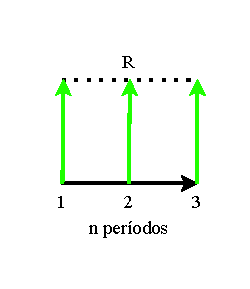
\includegraphics[height=5.3cm]{4_Capitulo/img/ejemplos/Exportados/Grafica 1.pdf}
        \end{center}

	\vspace{5mm}

	Para que la gráfica anterior represente una serie uniforme bien conformada es necesario agregarle un período que bien puede quedar al principio o al final. En el primer caso se tendrá:

        \vspace{5mm}
          \textbf{Gráfica 2}
          \\\\
        \textit{Ejemplo  representación de una serie}
	\begin{center}
       
		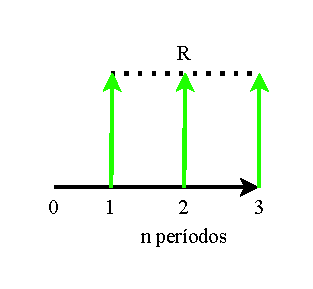
\includegraphics[height=5.3cm]{4_Capitulo/img/ejemplos/Exportados/Grafica 2.pdf}
        \end{center}
        \textit{Nota:}Este gráfico representa lo que  es una serie, bien conformada.Tomado de. Autoría propia.

	\vspace{5mm}

	La serie uniforme así conformada recibe el nombre de serie uniforme ordinaria o \textbf{serie uniforme vencida} que viene a ser aquella en que los pagos se efectúan al final del período, por ejemplo el pago de los sueldos de un empleado (primero viene el período de trabajo y después viene el pago).
	\\\\
	En el segundo caso se tendrá:

	\vspace{5mm}
         \textbf{Gráfica 3}
          \\\\
        
       \textit{ Ejemplo  representación de una serie anticipada}
        \begin{center}
		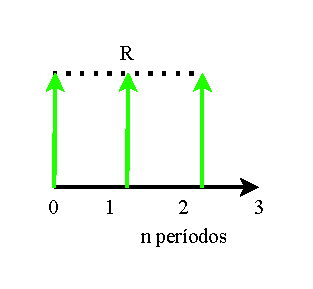
\includegraphics[height=5.3cm]{4_Capitulo/img/ejemplos/Exportados/Grafica 3.pdf}
        \end{center}
        \textit{Nota:}Este gráfico representa  una serie anticipada:Tomado de. Autoría propia
        \vspace{5mm}

        
	La serie uniforme así conformada recibe el nombre de \textbf{serie uniforme anticipada} porque los pagos se efectúan al principio del período, por ejemplo, el pago mensual del arriendo de una casa (primero paga y después tiene derecho a ocupar la casa durante el mes que pagó).
	\\\\

	\vspace{5mm}
 
       \textbf{Gráfica 4}
          \\\\
         \textit{Ejemplo  representación de una serie }
        \begin{center}
		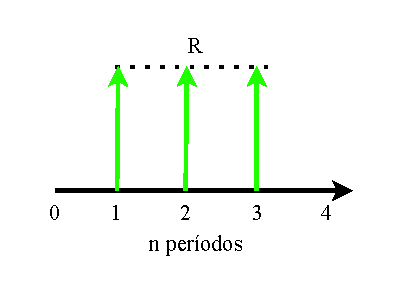
\includegraphics[height=5.3cm]{4_Capitulo/img/ejemplos/Exportados/Grafica 4.pdf}
        \end{center}
         \textit{Nota:}Este gráfico es una representación de lo que no es una serie.Tomado de. Autoria propia
        \vspace{5mm}
	

	Claramente puede observarse que cuando se inicia la gráfica con un ingreso y se termina con un ingreso como ocurre en la gráfica 1, no hay una serie uniforme bien conformada y cuando se inicia y finaliza la gráfica con ingreso como en el caso de la gráfica 4, tampoco hay una serie uniforme bien conformada. Las gráficas 2 y 3 si representan series periódicas bien conformadas y tienen una característica en común, que su inicio y fin son diferentes, en la gráfica 2 se inicia con período y se termina con ingreso y en la gráfica 3 se inicia con ingreso y se termina con período.
	\\\\
	En conclusión, para que una serie uniforme éste bien conformada su \textbf{inicio y fin deben ser diferentes.}

	\section{Plazo de una serie uniforme}
	El tiempo que transcurre entre el inicio del primer período y el final del último período se denomina período de la serie uniforme (mensual, trimestral, semestral, etc.)  y se representa por n.
	Una serie uniforme tiene dos valores, el valor final y el valor presente, en el primer caso todos los pagos son trasladados al final de la serie uniforme y en el segundo caso todos los pagos son trasladados al principio de la serie uniforme.

	\section{Valor futuro (VF, R, i, n)}
	El valor futuro se representa como VF
	\\\\
	En forma general se tendrá:

	\vspace{5mm}

        \textbf{Gráfica 5}
          \\\\
      
        \textit{Ejemplo valor futuro en series }
        \begin{center}
		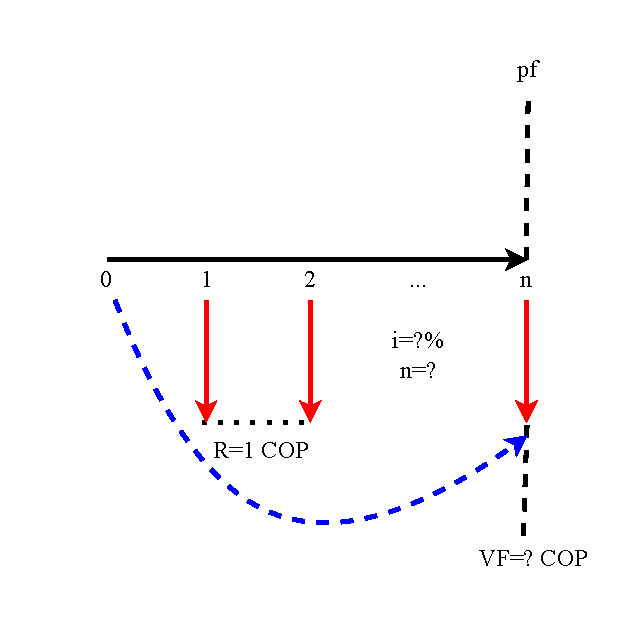
\includegraphics[scale=0.8]{4_Capitulo/img/ejemplos/Exportados/Grafica 5.pdf}
        \end{center}
        \textit{Nota:}Este gráfico es una representación del valor futuro en series. Autoria propia
        \vspace{5mm}
	

	Para plantear la ecuación de valor con período focal en \textbf n \textbf trasladamos cada uno de los pagos de 1 COP a valor final usando la ecuación del interés  compuesto.\\

        \begin{center}
        $F= P (1+i)^{n}$ \hspace{35pt}{Valor Futuro} \\
        \end{center}

	A cada pago, pero en cada caso, P = 1 COP. El pago que está en 1 se traslada por n-1 períodos y el que está en 2 se traslada por  n-2 períodos y así sucesivamente hasta llegar al pago que está en n  el cual no se traslada por estar  en la período focal, entonces:
 
        \begin{center}
	\begin{equation*}
		VF=1+ (1+i) +(1+i)^{2}+....+(1+i)^{n-1}  \ \ [1]
	\end{equation*}
         \end{center}

	Si la ecuación (1) se multiplica por (1+i) se obtiene la             ecuación (2), entonces:\\

        \begin{center}
        $VF(1+i)= (1+i) +(1+i)^{2}+....+(1+i)^{n} \ \ [2]$\\
        \end{center}

        Restando la ecuación (1) de la ecuación (2), se obtiene la ecuación (3):\\

        \begin{center}
	%begin{equation*}
	%	\begin{split}
    $VF(1+i)= (1+i)+(1+i)^{2}+...+(1+i)^{n}$ \ \ [1]
    	\\
    $VF=1+(1+i)+(1+i)^{2}+...+(1+i)^{n-1}$ \ \ [2]\\
    $VF (1+i) - VF = (1+i)^{n} -1$ \ \ [3]\\
    	%	\end{split}
	%\end{equation*}
        \end{center}

	Factorizando VF se obtiene la ecuación (4):\\
        \begin{center}
	%\begin{equation*}$VF(i)=(1+i)^{n}-1$ \ \ [4]\\ \\
	%\end{equation*}
         \end{center}
	Finalmente despejando VF se obtiene la ecuación (5):\\
        \begin{center}
	%\begin{equation*}

$VF = \frac {R((1+i)^n-1)}{i}$ \ \ [5] \hspace{35pt} {Valor futuro de una serie uniforme vencida} \\
	%\end{equation*}
          \end{center}

	\section{Valor presente (VP, R, i, n)}

	El caso del valor presente lo representaremos por VP. La fórmula se obtiene al plantear la ecuación de valor con período focal al principio y trasladando todos los pagos a valor presente con tasa i periódica vencida (nuevamente, no se pierde generalidad si se supone que todos los pagos o, ingresos son de 1 COP).

	\vspace{5mm}
         \textbf{Gráfica 6}
          \\\\
      
       \textit{Ejemplo de valor presente en series}
        \begin{center}
		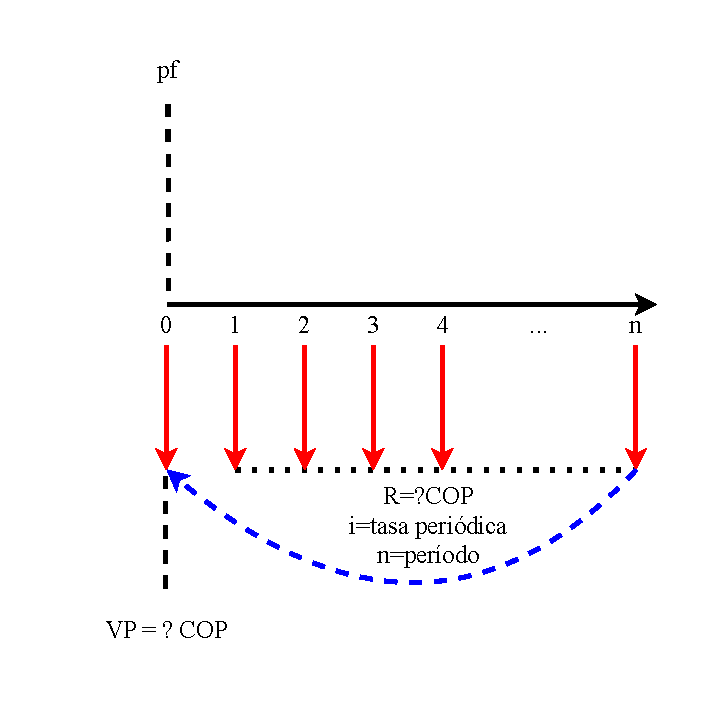
\includegraphics[scale=0.8]{4_Capitulo/img/ejemplos/Exportados/Grafica 6.pdf}
        \end{center}
        \textit{Nota:}Este gráfico es una representación del valor presente en series. Autoria propia
        \vspace{5mm}


    \begin{center}
   $VP=(1+i)^{-1}+(1+i)^{-2}+...+(1+i)^{-n}$\hspace{35pt} {Valor presente} \\
   
    \end{center}
    
	Para simplificar esta ecuación, podría seguirse un procedimiento similar al realizado para el valor final, sin embargo el camino más corto consiste en reemplazar el valor final.
	\\\\
 \begin{center}
$VP=VF(1+i)^{-n}$ \hspace{35pt} {Valor presente} \\
\end{center}

	Si $VF$ lo reemplazamos por su equivalente se tiene:
         \begin{center}
	%begin{equation*}
	$VP = R\frac{(1+i)^{n}-1}{i} (1+i)^{-n} = R\frac{1-(1+i)^{-n}}{i}$
	%end{equation*}
        \end{center}

	De donde se concluye que:
         \begin{center}
	%begin{equation*}
	$VP = R\frac{1-(1+i)^{-n}}{i}$\hspace{25pt} {  Valor presente de una serie uniforme vencida} \\
	%end{equation*}
        \end{center}
	Las fórmulas anteriores fueron deducidas para una renta de 1 COP pero si la renta hubiese sido de R COP, el valor final VF o el valor presente VP hubiese sido R veces mayor. Por tanto podemos escribir:
         \begin{center}
	%begin{align*}
		$VP=R \frac{1-(1+i)^{-n}}{i}$\hspace{35pt}{Valor presente serie uniforme vencida}

  \vspace{5mm}
		$VF=R \frac{(1+i)^{n}-1}{i}$\hspace{35pt}{Valor futuro serie uniforme vencida} 
	%end{align*}
\end{center}
 %%%%%%%%%%%%%%%%%%% EJERCICIO 2 %%%%%%

\textbf{Ejemplo 2}\\

Un documento estipula pagos trimestrales de 80.000 COP, durante 6 años. Si este documento se
cancelará con un solo pago de: A. al principio. B. al final. con una tasa del 32\% nominal
anual trimestre vencido. ¿Cuál será el valor que cancela al principio y al final?
\\

\textbf{Solución.}\\
%La tabla ira centrada
\begin{center}
	\renewcommand{\arraystretch}{1.5}% Margenes de las celdas
	%Creación de la cuadricula de 3 columnas
\begin{longtable}[H]{|c|c|c|}
		%Creamos una linea horizontal
\hline
		%Definimos el color de la primera fila
\rowcolor[HTML]{FFB183}
		%%%%% INICIO ASIGNACIÓN FECHA FOCAL %%%%%%%
		%%%%%%%%%% INICIO TITULO
		%Lo que se hace aquí es mezclar las 3 columnas en una sola
\multicolumn{3}{|c|}{\cellcolor[HTML]{FFB183}\textbf{1. Asignación período focal}}   \\ \hline
\multicolumn{3}{|c|} {$pf : 0 ptv$} \\ \hline
		%%%%%%%%%% FIN TITULO
  %%%%% INICIO DECLARACIÓN FORMULAS
  
%%%%%%%%%%% INICIO TITULO
\rowcolor[HTML]{FFB183}
\multicolumn{3}{|c|}{\cellcolor[HTML]{FFB183}\textbf{2. Declaración de variables}}    \\ \hline
%%%%%%%%%%% FIN TITULO
%%%%%%%%%%% INICIO MATEMÁTICAS
\multicolumn{1}{|c|}{\cellcolor[HTML]{FFB183}\textbf{Valores monetarios}}    & \multicolumn{1}{c|}{\cellcolor[HTML]{FFB183}\textbf{Valores no monetarios}} & \multicolumn{1}{c|}{\cellcolor[HTML]{FFB183}\textbf{Incógnitas}} \\ \hline
R = 80.000 COP & $j = 32\% natv \equiv 8\% ptv =i \hspace{0.3cm} $ & $VP = { ? } \hspace{0.3cm} COP  $ \\
& $n = 24 \textit{ ptv }$ & \\ \hline
%%%%%%%%%% FIN MATEMÁTICAS
		%%%%% INICIO FLUJO DE CAJA
\rowcolor[HTML]{FFB183}
\multicolumn{3}{|c|}{\cellcolor[HTML]{FFB183}\textbf{3. Diagrama de flujo de caja}} \\ \hline
		%Mezclamos 3 columnas y pondremos el dibujo
		%%%%%%%%%%%%% INSERCIÓN DE LA IMAGEN
		%Deberán descargar las imágenes respectivas del drive y pegarlas en la carpeta
		%n_capitulo/img/ejemplos/1/capitulo1ejemplo1.pdf  (el /1/ es el numero del ejemplo)
\multicolumn{3}{|c|}{ 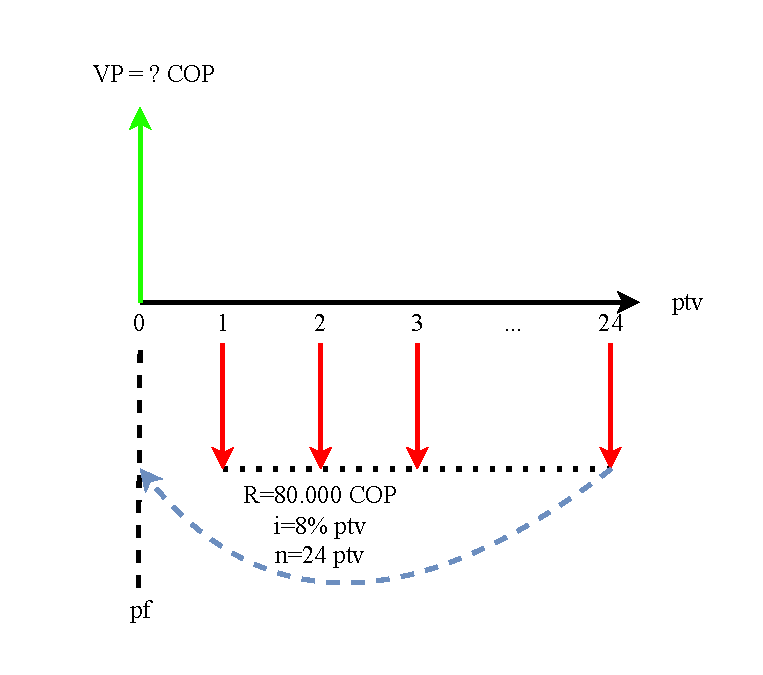
\includegraphics[scale=0.9, trim=-5 -5 -5 -5]{4_Capitulo/img/ejemplos/2/Exportados/Ejemplo 2A.pdf} }   
   \\ \hline
		%%%%%%%%%%%%% FIN INSERCIÓN DE IMAGEN
		%%%%%FIN FLUJO DE CAJA
		
		
		
		%%%%% INICIO DECLARACIÓN FORMULAS
		%%%%%%%%%%% INICIO TITULO
\rowcolor[HTML]{FFB183}
\multicolumn{3}{|c|}{\cellcolor[HTML]{FFB183}\textbf{4. Declaración de fórmulas}}    \\ \hline
		%%%%%%%%%%% FIN TITULO
		%%%%%%%%%%% INICIO MATEMÁTICAS
\multicolumn{3}{|c|} {$VP=R\frac{1-(1+i)^{-n}}{i}$ Valor presente serie uniforme vencida}   \\ \hline	
	
		%%%%%%%%%% FIN MATEMÁTICAS
		%%%%%% INICIO DESARROLLO MATEMÁTICO
\rowcolor[HTML]{FFB183}
		%%%%%%%%%%INICIO TITULO
\multicolumn{3}{|c|}{\cellcolor[HTML]{FFB183}\textbf{5. Desarrollo matemático}}       \\ \hline
		%%%%%%%%%% FIN TITULO
		%%%%%%%%%% INICIO MATEMÁTICAS
\multicolumn{3}{|c|}{ R = 80.000 \ $n = 24$\  $i=0.08$ \quad } \\
\multicolumn{3}{|c|}{VP= 80.000 COP $\frac{1-(1+0,08)^{-24}}{0,08}=$ 842.301,6627 COP}  \\
\multicolumn{3}{|c|}{VP= 842.301,6627 COP}  \\ \hline
		%%%%%%%%%% FIN MATEMÁTICAS
		%%%%%% FIN DESARROLLO MATEMÁTICO
		%%%%%% INICIO RESPUESTA
\rowcolor[HTML]{FFB183}
		%%%%%%%%%%INICIO TITULO
\multicolumn{3}{|c|}{\cellcolor[HTML]{FFB183}\textbf{6. Respuesta}}   \\ \hline
		%%%%%%%%%% FIN TITULO
		%%%%%%%%%% INICIO RESPUESTA MATEMÁTICA
\multicolumn{3}{|c|}{ El valor a cancelar al principio es de 842.302 COP }  \\ \hline
		
		
		%%%%%%%%%% FIN MATEMÁTICAS
		%%%%%% FIN RESPUESTA
	\end{longtable}
	%Se crean dos lineas en blanco para que no quede el siguiente texto tan pegado
	%\newline \newline %USARLO SI CREES QUE ES NECESARIO
\end{center}
%%%%%%%%%%%%%%%%%%%%%%%%%%FIN EJERCICIO 1 %%%%%%%%%%%%%%%%%%%%%%%%%%%


%\textbf{Tabla de rentabilidad en anual efectivo}\\

%%%%%%%%%%%%%%%%%%%%%%%%%%FIN EJERCICIO 2 %%%%%%%%%%%%%%%%%%%%%%%%%%%

 %%%%%%%%%%%%%%%%%%% EJERCICIO 2.2 %%%%%%

\textbf{Parte 2}\\



























\textbf{Solución.}\\
%La tabla ira centrada
\begin{center}
	\renewcommand{\arraystretch}{1.5}% Margenes de las celdas
	%Creación de la cuadricula de 3 columnas
\begin{longtable}[H]{|c|c|c|}
		%Creamos una linea horizontal
\hline
		%Definimos el color de la primera fila
\rowcolor[HTML]{FFB183}
		%%%%% INICIO ASIGNACIÓN FECHA FOCAL %%%%%%%
		%%%%%%%%%% INICIO TITULO
		%Lo que se hace aquí es mezclar las 3 columnas en una sola
\multicolumn{3}{|c|}{\cellcolor[HTML]{FFB183}\textbf{1. Asignación período focal}}   \\ \hline
\multicolumn{3}{|c|} {$pf : 24 ptv$} \\ \hline
		%%%%%%%%%% FIN TITULO
  %%%%% INICIO DECLARACIÓN FORMULAS

%%%%%%%%%%% INICIO TITULO
\rowcolor[HTML]{FFB183}
\multicolumn{3}{|c|}{\cellcolor[HTML]{FFB183}\textbf{2. Declaración de variables}}    \\ \hline
%%%%%%%%%%% FIN TITULO
%%%%%%%%%%% INICIO MATEMÁTICAS
\multicolumn{1}{|c|}{\cellcolor[HTML]{FFB183}\textbf{Valores monetarios}}    & \multicolumn{1}{c|}{\cellcolor[HTML]{FFB183}\textbf{Valores no monetarios}} & \multicolumn{1}{c|}{\cellcolor[HTML]{FFB183}\textbf{Incógnitas}} \\ \hline
R = 80.000 COP & $j = 32\% natv \equiv 8\% ptv =i \hspace{0.3cm} $ & $VF = { ? } \hspace{0.3cm} COP  $ \\
& $n = 24 \textit{ ptv }$ & \\ \hline
%%%%%%%%%% FIN MATEMÁTICAS
		%%%%% INICIO FLUJO DE CAJ
\rowcolor[HTML]{FFB183}
\multicolumn{3}{|c|}{\cellcolor[HTML]{FFB183}\textbf{3. Diagrama de flujo de caja}} \\ \hline
		%Mezclamos 3 columnas y pondremos el dibujo
		%%%%%%%%%%%%% INSERCIÓN DE LA IMAGEN
		%Deberán descargar las imágenes respectivas del drive y pegarlas en la carpeta
		%n_capitulo/img/ejemplos/1/capitulo1ejemplo1.pdf  (el /1/ es el numero del ejemplo)
\multicolumn{3}{|c|}{ 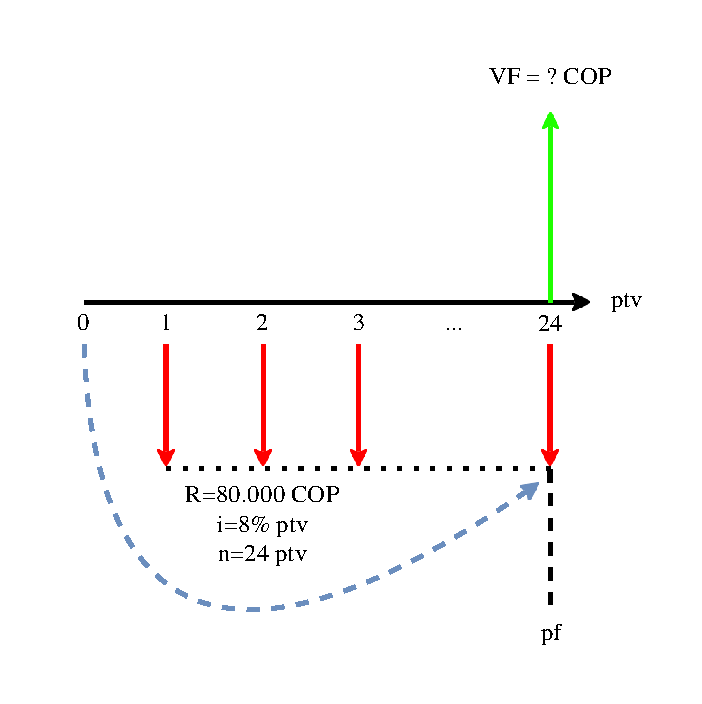
\includegraphics[scale=0.8, trim=-5 -5 -5 -5]{4_Capitulo/img/ejemplos/2.2/Exportados/Ejemplo 2B.pdf} }   
   \\ \hline
		%%%%%%%%%%%%% FIN INSERCIÓN DE IMAGEN
		%%%%%FIN FLUJO DE CAJA



		%%%%% INICIO DECLARACIÓN FORMULAS
		%%%%%%%%%%% INICIO TITULO
\rowcolor[HTML]{FFB183}
\multicolumn{3}{|c|}{\cellcolor[HTML]{FFB183}\textbf{4. Declaración de fórmulas}}    \\ \hline
		%%%%%%%%%%% FIN TITULO
		%%%%%%%%%%% INICIO MATEMÁTICAS
\multicolumn{3}{|c|} {$VF=R\frac{(1+i)^{n}-1}{i}$ Valor futuro serie uniforme vencida}   \\ \hline

		%%%%%%%%%% FIN MATEMÁTICAS
		%%%%%% INICIO DESARROLLO MATEMÁTICO
\rowcolor[HTML]{FFB183}
		%%%%%%%%%%INICIO TITULO
\multicolumn{3}{|c|}{\cellcolor[HTML]{FFB183}\textbf{5. Desarrollo matemático}}       \\ \hline
		%%%%%%%%%% FIN TITULO
		%%%%%%%%%% INICIO MATEMÁTICAS
\multicolumn{3}{|c|}{ R = 80.000 \ $n = 24$\  $i=0.08$ \quad } \\
\multicolumn{3}{|c|}{VF=80.000 COP $\frac{(1+0,08)^{24}-1}{0,08}=$ 5.341.180,737 COP}  \\
\multicolumn{3}{|c|}{VF= 5.341.180,737 COP}  \\ \hline

		%%%%%%%%%% FIN MATEMÁTICAS
		%%%%%% FIN DESARROLLO MATEMÁTICO
		%%%%%% INICIO RESPUESTA
\rowcolor[HTML]{FFB183}
		%%%%%%%%%%INICIO TITULO
\multicolumn{3}{|c|}{\cellcolor[HTML]{FFB183}\textbf{6. Respuesta}}   \\ \hline
		%%%%%%%%%% FIN TITULO
		%%%%%%%%%% INICIO RESPUESTA MATEMÁTICA
\multicolumn{3}{|c|}{ El valor a cancelar al final es de 5.341.181 COP }  \\ \hline


		%%%%%%%%%% FIN MATEMÁTICAS
		%%%%%% FIN RESPUESTA
	\end{longtable}
	%Se crean dos lineas en blanco para que no quede el siguiente texto tan pegado
	%\newline \newline %USARLO SI CREES QUE ES NECESARIO
\end{center}
%%%%%%%%%%%%%%%%%%%%%%%%%%FIN EJERCICIO 1 %%%%%%%%%%%%%%%%%%%%%%%%%%%


%\textbf{Tabla de rentabilidad en anual efectivo}\\

%%%%%%%%%%%%%%%%%%%%%%%%%%FIN EJERCICIO 2.2 %%%%%%%%%%%%%%%%%%%%%%%%%%%


%%%%%%%%%%%%%%%%%%% EJERCICIO 3 %%%%%%

\textbf{Ejemplo 3}\\

Una persona empieza el día primero de julio de 1986 a hacer depósitos de 1.000.000 COP
mensualmente el día primero de cada mes. Estos depósitos son efectuados en una entidad
financiera que le paga el 24\% nominal anual mes vencido; pero a partir del primero de
octubre de 1987 [15 períodos mensuales], decidió que de ahí en adelante sus depósitos serían de 2.500.000 COP,
el último depósito lo hizo el primero de agosto de 1989. Si el primero de diciembre de 1989
decide cancelar la cuenta. ¿Cuál será el monto de sus ahorros?
\\

\textbf{Solución.}\\
%La tabla ira centrada
\begin{center}
	\renewcommand{\arraystretch}{1.5}% Margenes de las celdas
	%Creación de la cuadricula de 3 columnas
\begin{longtable}[H]{|c|c|c|}
		%Creamos una linea horizontal
\hline
		%Definimos el color de la primera fila
\rowcolor[HTML]{FFB183}
		%%%%% INICIO ASIGNACIÓN FECHA FOCAL %%%%%%%
		%%%%%%%%%% INICIO TITULO
		%Lo que se hace aquí es mezclar las 3 columnas en una sola
\multicolumn{3}{|c|}{\cellcolor[HTML]{FFB183}\textbf{1. Asignación período focal}}   \\ \hline
\multicolumn{3}{|c|} {$pf : 42 pmv$} \\ \hline
		%%%%%%%%%% FIN TITULO
  %%%%% INICIO DECLARACIÓN FORMULAS
  
%%%%%%%%%%% INICIO TITULO
\rowcolor[HTML]{FFB183}
\multicolumn{3}{|c|}{\cellcolor[HTML]{FFB183}\textbf{2. Declaración de variables}}    \\ \hline
%%%%%%%%%%% FIN TITULO
%%%%%%%%%%% INICIO MATEMÁTICAS
\multicolumn{1}{|c|}{\cellcolor[HTML]{FFB183}\textbf{Valores monetarios}}    & \multicolumn{1}{c|}{\cellcolor[HTML]{FFB183}\textbf{Valores no monetarios}} & \multicolumn{1}{c|}{\cellcolor[HTML]{FFB183}\textbf{Incógnitas}} \\ \hline
$R_{1}$ = 1.000.000 COP & $j = 24\% namv \equiv 2\% pmv=i$ & VF = ? COP \\
$R_{3}$ = 2.500.000 COP & $ n_{1} = 15 pmv $& \\
& $ n_{2} = 27 pmv $  & \\
& $ n_{3} = 23 pmv $ & \\
& $ n_{4} = 4 pmv $ & \\ \hline
%%%%%%%%%% FIN MATEMÁTICAS
		%%%%% INICIO FLUJO DE CAJA
\rowcolor[HTML]{FFB183}
\multicolumn{3}{|c|}{\cellcolor[HTML]{FFB183}\textbf{3. Diagrama de flujo de caja}} \\ \hline
		%Mezclamos 3 columnas y pondremos el dibujo
		%%%%%%%%%%%%% INSERCIÓN DE LA IMAGEN
		%Deberán descargar las imágenes respectivas del drive y pegarlas en la carpeta
		%n_capitulo/img/ejemplos/1/capitulo1ejemplo1.pdf  (el /1/ es el numero del ejemplo)
\multicolumn{3}{|c|}{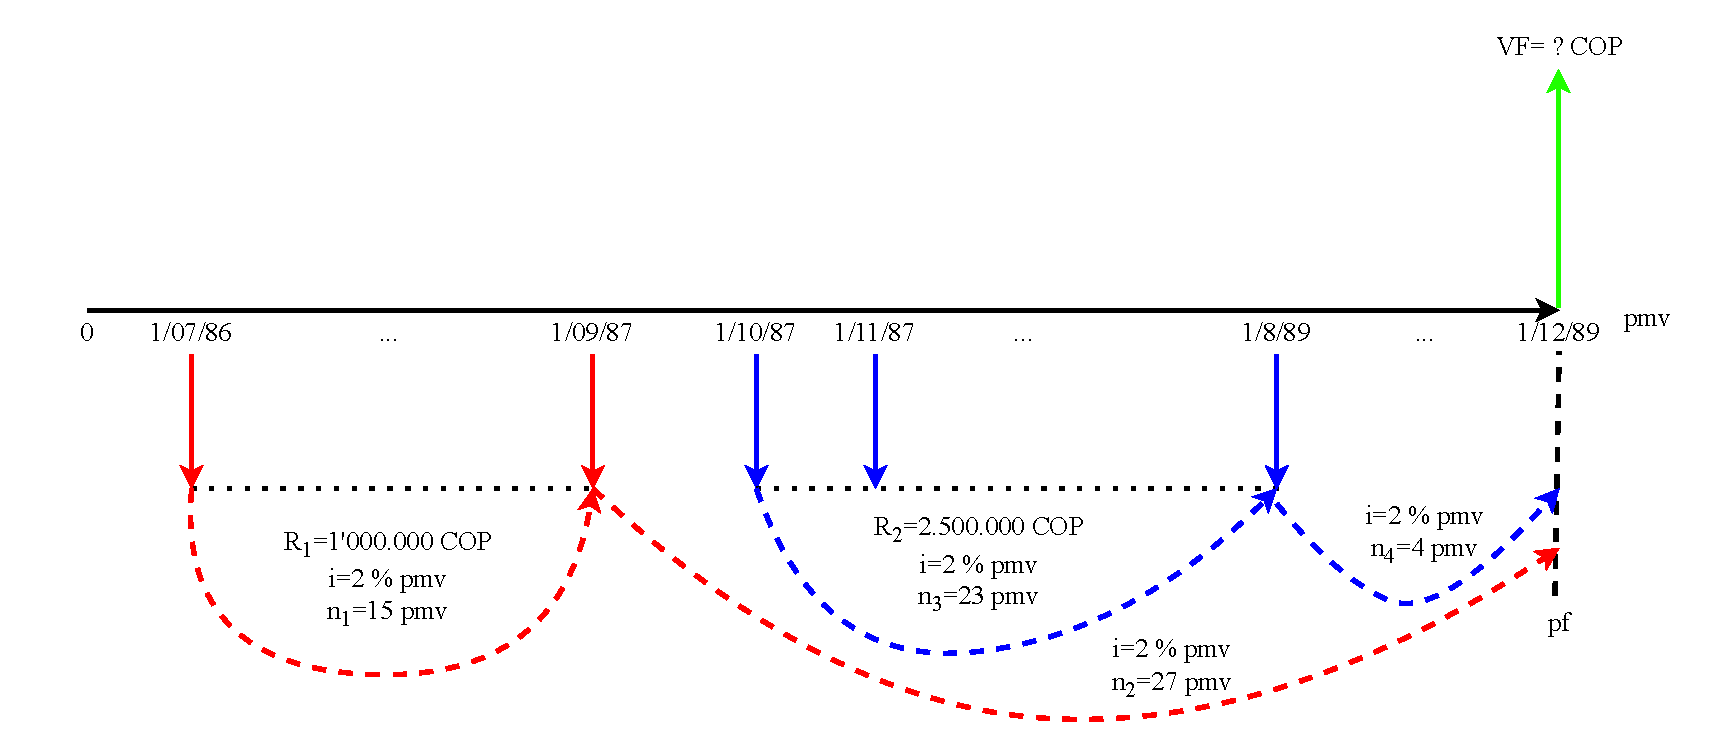
\includegraphics[scale=0.5, trim=-5 -5 -10 -10]{4_Capitulo/img/ejemplos/3/Exportados/Ejemplo 3.pdf} }   
   \\ \hline
		%%%%%%%%%%%%% FIN INSERCIÓN DE IMAGEN
		%%%%%FIN FLUJO DE CAJA
		
		
		
		%%%%% INICIO DECLARACIÓN FORMULAS
		%%%%%%%%%%% INICIO TITULO
\rowcolor[HTML]{FFB183}
\multicolumn{3}{|c|}{\cellcolor[HTML]{FFB183}\textbf{4. Declaración de fórmulas}}    \\ \hline
		%%%%%%%%%%% FIN TITULO
		%%%%%%%%%%% INICIO MATEMÁTICAS
\multicolumn{3}{|c|} {$VF=R\frac{(1+i)^{n}-1}{i}$ Valor futuro serie uniforme vencida}   \\ \hline	
	
		%%%%%%%%%% FIN MATEMÁTICAS
		%%%%%% INICIO DESARROLLO MATEMÁTICO
\rowcolor[HTML]{FFB183}
		%%%%%%%%%%INICIO TITULO
\multicolumn{3}{|c|}{\cellcolor[HTML]{FFB183}\textbf{5. Desarrollo matemático}}       \\ \hline
		%%%%%%%%%% FIN TITULO
		%%%%%%%%%% INICIO MATEMÁTICAS
\multicolumn{3}{|c|}		
{VF=1.000.000 COP $\frac{(1+0,02)^{15}-1}{0,02}\textcolor{red}*[1+0.02]^{27} +$ 2.500.000 COP $\frac{(1+0.02)^{23}-1}{0.02}\textcolor{red}*[1+0.02]^{4}$}\\
\multicolumn{3}{|c|}	
{VF = 107.574.001 COP}\\ \hline
		
		%%%%%%%%%% FIN MATEMÁTICAS
		%%%%%% FIN DESARROLLO MATEMÁTICO
		%%%%%% INICIO RESPUESTA
\rowcolor[HTML]{FFB183}
		%%%%%%%%%%INICIO TITULO
\multicolumn{3}{|c|}{\cellcolor[HTML]{FFB183}\textbf{6. Respuesta}}   \\ \hline
		%%%%%%%%%% FIN TITULO
		%%%%%%%%%% INICIO RESPUESTA MATEMÁTICA
\multicolumn{3}{|c|}{ El monto de sus ahorros será de 107.574.001 COP }  \\ \hline
		
		
		%%%%%%%%%% FIN MATEMÁTICAS
		%%%%%% FIN RESPUESTA
	\end{longtable}
	%Se crean dos lineas en blanco para que no quede el siguiente texto tan pegado
	%\newline \newline %USARLO SI CREES QUE ES NECESARIO
\end{center}
%%%%%%%%%%%%%%%%%%%%%%%%%%FIN EJERCICIO 3 %%%%%%%%%%%%%%%%%%%%%%%%%%%


%\textbf{Tabla de rentabilidad en anual efectivo}\\

%%%%%%%%%%%%%%%%%%%%%%%%%%FIN EJERCICIO 3 %%%%%%%%%%%%%%%%%%%%%%%%%%%

	

	\section{Series periódicas anticipadas (VP, VF, R, i, n)}

	Una serie uniforme anticipada es aquella en que los pagos se hacen al principio del período. El valor presente y el valor futuro se representarán respectivamente por: $VP_{a}$ y $VF_{a}$.

\begin{center}

$VF_{a}=R \frac{(1+i)^{n}-1}{i}(1+i) $ \hspace{35pt}{ Valor  futuro de una serie  uniforme  anticipada}

$VP_{a}=R \frac{1-(1+i)^{(-n)}}{i}(1+i)$
	\hspace{30pt}{Valor de una presente  serie  uniforme  anticipada}\\
 \end{center}	


	Existen relaciones entre las series periódicas vencidas y las series periódicas anticipadas, las cuales serán deducidas del análisis de las series uniformes vencidas: Para facilitar el planteamiento de la ecuación de valor se comienza con el flujo que está en n, siguiendo con el que está en n-1 y así sucesivamente hasta llegar al pago situado en 1, entonces para valor final con serie uniforme la ecuación de equivalencia quedará así:

	\vspace{5mm}
\begin{center}
$VF_{a}=1+ (1+i) +(1+i)^{2}+...+(1+i)^{n} $ \\

\end{center}

\textbf{Demostración:}
Queremos demostrar la fórmula de la suma de los términos:
\[
VF_{a} = 1 + (1+i) + (1+i)^2 + \dots + (1+i)^n
\]

Esta expresión es una progresión geométrica con \(n+1\) términos, donde el primer término (\(a\)) es \(1\) y la razón común (\(r\)) es \(1+i\).

La fórmula general para la suma de una progresión geométrica finita es:
\[
S = a \cdot \frac{1 - r^N}{1 - r}, \quad \text{para } r \neq 1.
\]

Sustituyendo los valores:
\[
a = 1, \quad r = 1+i, \quad N = n+1.
\]

Por lo tanto, la suma se expresa como:
\[
VF_{a} = 1 \cdot \frac{1 - (1+i)^{n+1}}{1 - (1+i)}.
\]

Simplificamos el denominador:
\[
1 - (1+i) = -i.
\]

Sustituyendo, obtenemos:
\[
VF_{a} = \frac{1 - (1+i)^{n+1}}{-i}.
\]

Multiplicamos numerador y denominador por \(-1\) para simplificar:
\[
VF_{a} = \frac{(1+i)^{n+1} - 1}{i}.
\]

Por lo tanto, la fórmula final es:
\[
VF_{a} = \frac{(1+i)^{n+1} - 1}{i}.
\]

	\vspace{5mm}

	\textbf{Serie uniforme vencida:}
	\vspace{5mm}
        \textbf{Gráfica 7}
          \\\\
        \textit{Ejemplo representación serie uniforme vencida }
        \begin{center}
		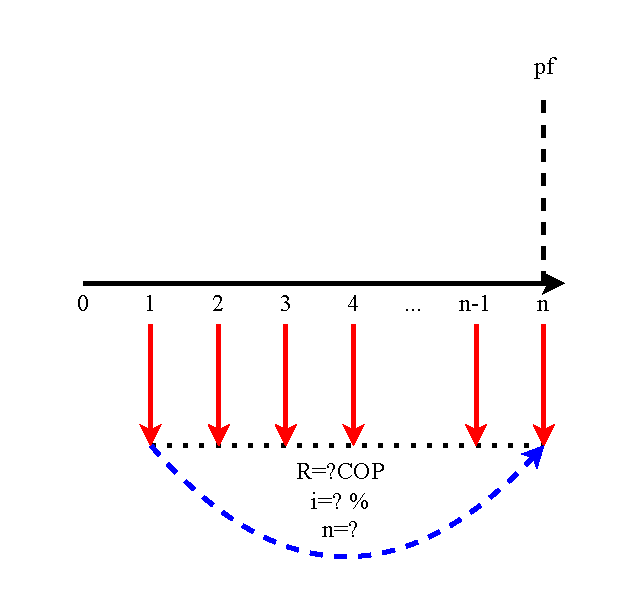
\includegraphics[scale=0.8]{4_Capitulo/img/ejemplos/Exportados/Grafica 7.pdf}
        \end{center}
    \textit{Nota:}Este gráfico es una representación serie uniforme vencida. Autoria propia
        \vspace{5mm}

	

	Para la serie uniforme vencida en valor final, la gráfica del flujo de caja quedará así:
	\textbf{\\ \\ Serie uniforme anticipada:}
	\vspace{5mm}
        \textbf{Gráfica 8}
        \\ \\
    
        \textit{Ejemplo representacion serie uniforme anticipada}
        \begin{center}
		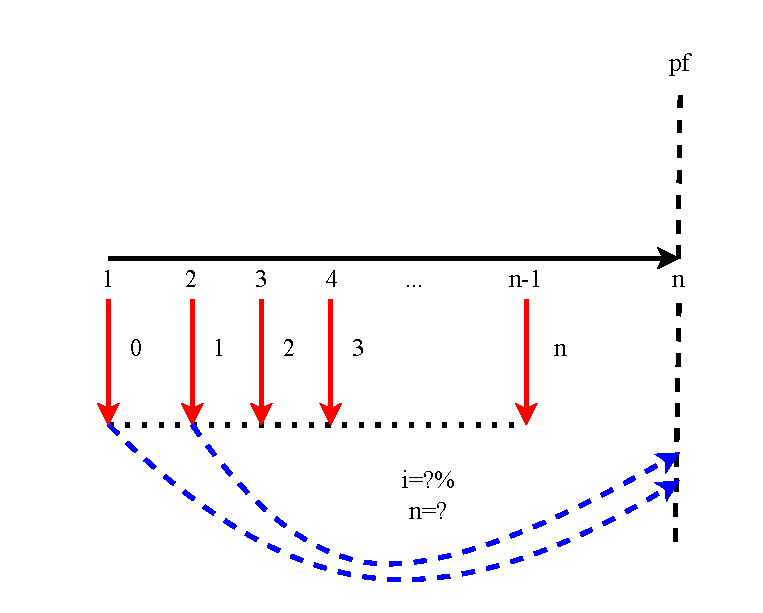
\includegraphics[scale=0.8]{4_Capitulo/img/ejemplos/Exportados/Grafica 8.pdf}
        \end{center}
        \textit{Nota:}Este gráfico es una representación serie uniforme anticipada. Autoria propia
        \vspace{5mm}
	
	Observe que en este caso se ha usado una doble numeración, la que está encima de la línea de tiempo indica el número del pago, mientras que la que se encuentra debajo de la línea de tiempo señala los períodos. \\

	En el período 0 que es el comienzo del primer período, se está haciendo el pago número 1, en el período 1 que es el final del primer período pero a su vez es el comienzo del segundo período y por eso se realiza el segundo pago y así sucesivamente hasta que se llega al punto n-1. La ecuación de equivalencia para la anterior situación será:\\\\
	\vspace{5mm}
 \begin{center}
$VF_{a}=(1+i)^{1}  +(1+i)^{2}+...+(1+i)^{n-1}+(1+i)^{n}$
\end{center}
	\vspace{5mm}
	Donde:

		
		  $VF_a =$ es el valor futuro anticipado al final del último período.

		  $i =$ es la tasa de interés por período.

		  Los términos $(1+i)^k$ = representan el crecimiento acumulado de cada pago al final del período \(n\), con \(k\) variando de 1 a \(n\).
		  \vspace{5mm}
		  Esta es una serie geométrica en la que:

		  \begin{itemize}
			\item El primer término es \((1+i)^1\),
			\item La razón común es \((1+i)\),
			\item El número total de términos es \(n\).
		  \end{itemize}

		\vspace{5mm}
	
	
	
	La diferencia entre las dos series periódicas consiste en que la serie de la serie uniforme vencida empieza con 1 y termina con $(1+i)^{(n-1)}$, en cambio, la serie de la serie uniforme anticipada comienza con $(1+i)$  y termina con $(1+i)^{n}$. Si a la serie anticipada se le agrega un 1 y se le resta al final y, si además, le introducimos el paréntesis angular, el resultado no se altera.

	\vspace{5mm}
 \begin{center}
$VFa=[1+(1+i) +(1+i)^{2}+(1+i)^{3}...+(1+i)^{(n-1)} ]+(1+i)^{n} -1$
\end{center}
	\vspace{5mm}

	Obsérvese que la parte que está dentro del paréntesis es igual a la serie uniforme vencida, por tanto, podemos decir que:

	\vspace{5mm}
 \begin{center}
$VFa=VF+(1+i)^{n}-1$
\end{center}
	\vspace{5mm}

	Si reemplazamos VF por su equivalente $\frac{(1+i)^{n}-1}{i}$ se tendrá:

	\vspace{5mm}
 \begin{center}
	VF$_{a}$=$\frac{(1+i)^{n}-1}{i}$+$i\frac{(1+i)^{n}-1}{i}$
 \end{center}
	\vspace{5mm}

	Si se factoriza  $\frac{(1+i)^{n}-1}{i}$, se tendrá:

	\vspace{5mm}
 \begin{center}
	VF$_{a}$=$\frac{(1+i)^{n}-1}{i}$(1+i) \ \  Pero \ \ como \ \ $VF = \frac{(1+i)^{n}-1}{i}$
 \end{center}
	\vspace{5mm}

	Entonces se tiene que:

	\vspace{5mm}
 \begin{center}
$VF_{a}=\frac{(1+i)^{n}-1}{i}(1+i) = VF (1+i)$  \hspace{35pt}{ Valor  futuro  serie  uniforme  anticipada}
\end{center}

	\vspace{5mm}

%%%%%%%%%%%%%%%%%%% EJERCICIO 4 %%%%%%

%%%%%%%%%% NO OLVIDAR COLOCAR ESTE COMENTARIO CON EL NUMERO DE EJERCICIO %%%%%%%%%%%%%
%%%%%%%%%%%%%%%%%%% EJERCICIO 5 %%%%%%
%%Text bf para negrilla , el \\ es para el salto de linea.
%%El primer \\ hace un espacio en el texto y el 2 \\ crea otro espacio
\textbf{Ejemplo 4}\newline
Una persona arrienda una casa en 50.000 COP pagaderos por mes anticipado, Si tan pronto como recibe cada arriendo, lo invierte en un fondo que le paga el 2\% periodo mes anticipado ¿Cuál será el monto de sus ahorros al final de un año?\\ \\

\textbf{Solución.}\\
\begin{center}

	\renewcommand{\arraystretch}{1.5}% Margenes de las celdas
	%Creación de la cuadricula
	\begin{longtable}{|c|c|c| }
		%Creamos una linea horizontal
		\hline
		%Definimos el color de la primera fila
		\rowcolor[HTML]{FFB183}
		%%%%% INICIO ASIGNACIÓN FECHA FOCAL %%%%%%%
		%%%%%%%%%% INICIO TITULO
		%Lo que se hace aquí es mezclar las 3 columnas en una sola
		\multicolumn{3}{|c|}{\cellcolor[HTML]{FFB183}\textbf{1. Asignación período focal}}   \\ \hline
		%%%%%%%%%% FIN TITULO
		%%%%% INICIO DECLARACIÓN DE VARIABLES %%%%%%%
		\multicolumn{3}{|c|}{$pf : 12pma$} \\ \hline
		%Definimos el color de la primera fila
		\rowcolor[HTML]{FFB183}
		%%%%% INICIO DECLARACIÓN DE VARIABLES %%%%%%%
		%%%%%%%%%% INICIO TITULO
		\multicolumn{3}{|c|}{\cellcolor[HTML]{FFB183}\textbf{2. Declaración de variables}}                                                                                   \\ \hline
		%%%%%%%%%% FIN TITULO
		%%%%%%%%%% INICIO DE MATEMÁTICAS
		\multicolumn{1}{|c|}{\cellcolor[HTML]{FFB183}\textbf{Valores monetarios}}    & \multicolumn{1}{c|}{\cellcolor[HTML]{FFB183}\textbf{Valores no monetarios}} & \multicolumn{1}{c|}{\cellcolor[HTML]{FFB183}\textbf{Incógnitas}} \\ \hline
		R = 50.000 COP  & $n = 12 pma$ & VF = ? COP  \\
		& $i=2\% pma$ & \\ \hline
		%%%%%%%%%% FIN DE MATEMÁTICAS
		%%%%% FIN DECLARACIÓN DE VARIABLES


		%%%%% INICIO FLUJO DE CAJA
		\rowcolor[HTML]{FFB183}
		\multicolumn{3}{|c|}{\cellcolor[HTML]{FFB183}\textbf{3. Diagrama de flujo de caja}}                                                                                  \\ \hline
		%Mezclamos 3 columnas y pondremos el dibujo
		%%%%%%%%%%%%% INSERCIÓN DE LA IMAGEN
		\multicolumn{3}{|c|}{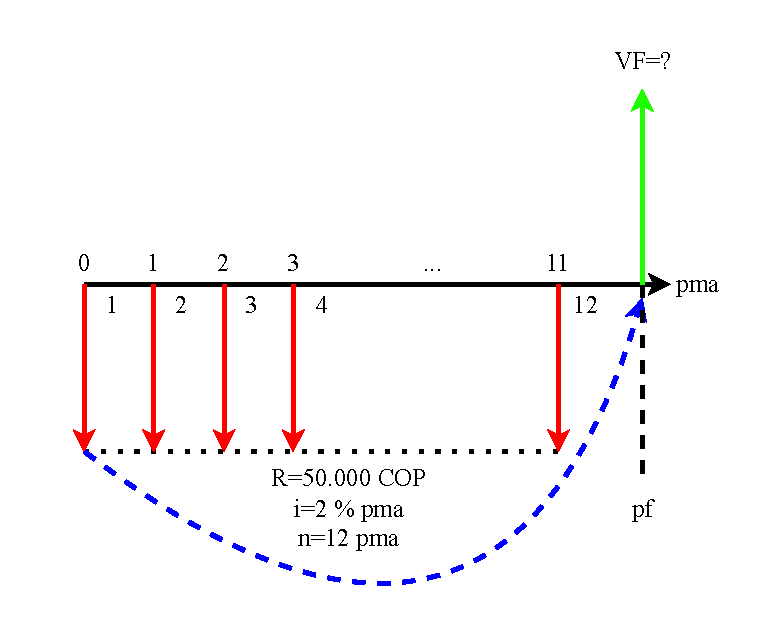
\includegraphics[scale=1,trim=-5 -5 -15 -5]{4_Capitulo/img/ejemplos/5/Exportados/Ejemplo 4.pdf} }                                                                                         \\ \hline
		%%%%%%%%%%%%% FIN INSERCIÓN DE IMAGEN
		%%%%%FIN FLUJO DE CAJA



		%%%%% INICIO DECLARACIÓN FORMULAS
		%%%%%%%%%%% INICIO TITULO
		\rowcolor[HTML]{FFB183}
		\multicolumn{3}{|c|}{\cellcolor[HTML]{FFB183}\textbf{4. Declaración de fórmulas}}                                                                                    \\ \hline
		%%%%%%%%%%% FIN TITULO
		%%%%%%%%%%% INICIO MATEMÁTICAS

		 \multicolumn{3}{|c|}{$VF_a=R \frac{(1+i)^{n}-1}{i}(1+i)$ \hspace{0.3cm} {Valor futuro serie uniforme anticipada}}                                                           \\ \hline
		%%%%%%%%%% FIN MATEMÁTICAS
		%%%%%% INICIO DESARROLLO MATEMÁTICO
		\rowcolor[HTML]{FFB183}
		%%%%%%%%%%INICIO TITULO
		\multicolumn{3}{|c|}{\cellcolor[HTML]{FFB183}\textbf{5. Desarrollo matemático}}                                                                                      \\ \hline
		%%%%%%%%%% FIN TITULO
		%%%%%%%%%% INICIO MATEMÁTICAS
		\multicolumn{3}{|c|}{ R = 50.000 \ $n = 12$\  $i=0.02$ \quad } \\
		\multicolumn{3}{|c|}{$VF_{a}=$50.000 COP$\frac{(1+0,02)^{12}-1}{0,02}\textcolor{red}*(1+0,02)$}\\                               
		\multicolumn{3}{|c|}{$VF_{a}$=684.016,58 COP }                               \\ \hline
		%%%%%%%%%% FIN MATEMÁTICAS
		%%%%%% FIN DESARROLLO MATEMÁTICO

		\rowcolor[HTML]{FFB183}
		\multicolumn{3}{|c|}{\cellcolor[HTML]{FFB183}\textbf{6. Respuesta}}    \\ \hline

		\multicolumn{3}{|c|}{El monto de sus ahorros al final de año será de 684.017 COP} \\ \hline
	\end{longtable}
	%Se crean dos lineas en blanco para que no quede el siguiente texto tan pegado
	%\newline \newline
\end{center}
%%%%%%%%%%%%%%%%%%%%%%%%%%FIN EJERCICIO X %%%%%%%%%%%%%%%%%%%%%%%%%%%

%%%%%%%%%%%%%%%%%%%%%%%%%%FIN EJERCICIO 4%%%%%%%%%%%%%%%%%%%%%%%%%%%



	\section{Valor presente de las series uniformes anticipada}

	La diferencia entre las series uniformes vencidas y las anticipadas consiste en que las primeras comienzan con $1$ y termina con $(1+i)^{-n}$ y la anticipada comienza con $1$ y termina con $(1+i)^{-(n-1)}$.

\vspace{5mm}	
\textbf{Gráfica 9}
        \\ \\
     
 \textit{Ejemplo representacion valor presente series uniformes anticipadas }
 \begin{center}
		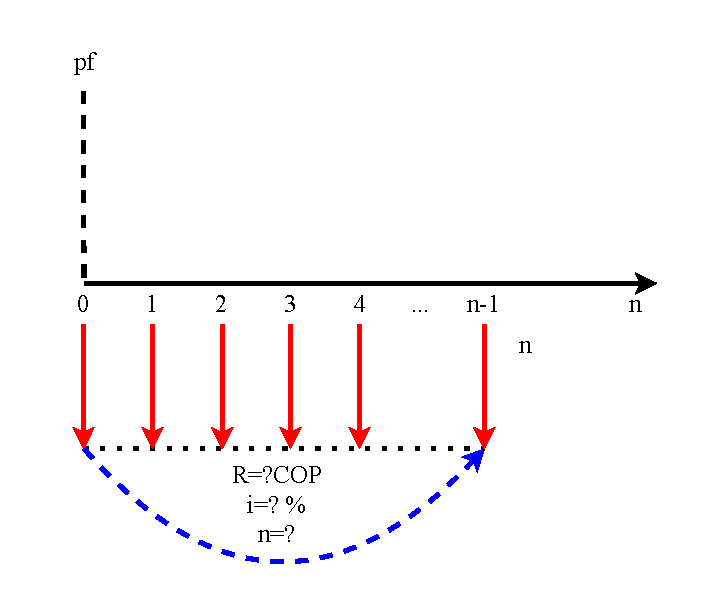
\includegraphics[scale=0.8]{4_Capitulo/img/ejemplos/Exportados/Grafica 9.pdf}
  \end{center}
  \textit{Nota:}Este gráfico es una representación del valor presente de las  series uniforme anticipada. Autoria propia
   \vspace{5mm}      
	

	Y la correspondiente ecuación de valor quedará así:\\
	\begin{center}

		$VP_{a}=1+[(1+i)^{-1}+(1+i)^{-2}+...+(1+i)^{-(n-1)} ] -(1+i)^{-n}$

	\end{center}

	\textbf{Demostración de la ecuación de valor para una serie uniforme anticipada}

	En una serie uniforme anticipada, los pagos comienzan al inicio del primer periodo y terminan al inicio del último periodo. Por tanto:

	\[
	\text{Valor presente anticipado } (VP_a) = 1 + \sum_{k=1}^{n-1} (1 + i)^{-k}
	\]

	El término \(1\) representa el valor presente del primer pago inmediato, y la suma es el valor presente de los pagos diferidos que comienzan en el segundo periodo.

	Descomposición de la suma:
	La suma \(\sum_{k=1}^{n-1} (1+i)^{-k}\) es una serie geométrica finita de la forma:

	\[
	S = a + ar + ar^2 + \ldots + ar^{n-1}
	\]

	Donde:
	\begin{itemize}
		\item \(a = (1+i)^{-1}\),
		\item \(r = (1+i)^{-1}\),
		\item El número de términos es \(n-1\).
	\end{itemize}

	La suma de una serie geométrica finita está dada por:
	\[
	S = a \frac{1 - r^n}{1 - r}
	\]

	Sustituyendo:
	\[
	S = (1+i)^{-1} \frac{1 - \left[(1+i)^{-1}\right]^{n-1}}{1 - (1+i)^{-1}}
	\]

	Simplificando el denominador \(1 - (1+i)^{-1}\):
	\[
	1 - (1+i)^{-1} = \frac{(1+i) - 1}{1+i} = \frac{i}{1+i}
	\]

	Entonces, la suma es:
	\[
	S = \frac{(1+i)^{-1} \cdot \left[1 - (1+i)^{-(n-1)}\right]}{\frac{i}{1+i}}
	\]

	Multiplicamos por el inverso del denominador:
	\[
	S = \frac{(1+i)^{-1} \cdot \left[1 - (1+i)^{-(n-1)}\right] \cdot (1+i)}{i}
	\]

	Cancelamos términos similares:
	\[
	S = \frac{\left[1 - (1+i)^{-(n-1)}\right]}{i}
	\]

	\textbf{Valor presente anticipado}
	El valor presente anticipado incluye el primer pago inmediato (\(1\)) y la suma de los valores presentes de los \(n-1\) pagos restantes. Por lo tanto:

	\[
	VP_a = 1 + \frac{1 - (1+i)^{-(n-1)}}{i}
	\]


	Ahora si a la serie de la serie uniforme anticipada le agregamos $(1+i)^{-n}$, le restamos esa misma cantidad y además le introducimos un paréntesis angular, el resultado no se altera entonces:

	\vspace{5mm}
\begin{center}
$VP_{a}= 1+[(1+i)^{-1} +(1+i)^{-2}+...+(1+i)^{-(n-1)} +(1+i)^{-n} ] -(1+i)^{-n}$
\end{center}
	\vspace{5mm}
	Ahora podemos observar que la serie que está dentro del paréntesis angular corresponde a la serie ordinaria, por tanto podemos decir que:

	\vspace{5mm}
\begin{center}
$VP_{a}= 1+VP-(1+i)^{-n}=VP+1-(1+i)^{-n}$
	\vspace{5mm}
\end{center}
	Si los dos últimos términos de la ecuación anterior se encierran en un paréntesis angular y se multiplican y dividiendo por i, no se altera la igualdad, por tanto se tiene:

	\vspace{5mm}
 \begin{center}
$VP_{a}=VP+\frac{i (1-i)^{-n} }{i}=VP+iVP$
\end{center}
	\vspace{5mm}

	Factorizando VP se tiene la fórmula final

	\vspace{5mm}
 \begin{center}
$VP_{a}=VP \frac{1-(1+i)^{-n}}{i}(1+i)$ \hspace{35pt}{Valor presente de una serie uniforme anticipada}\\
\end{center}
	\vspace{5mm}
%%%%%%%%%%%%%%%%%%% EJERCICIO 5 %%%%%%

%%%%%%%%%% NO OLVIDAR COLOCAR ESTE COMENTARIO CON EL NUMERO DE EJERCICIO %%%%%%%%%%%%%
%%%%%%%%%%%%%%%%%%% EJERCICIO 7 %%%%%%
%%Text bf para negrilla , el \\ es para el salto de linea.
%%El primer \\ hace un espacio en el texto y el 2 \\ crea otro espacio
\textbf{Ejemplo 5}\newline
El contrato de arriendo de una casa estipula pagos mensuales de 40.000 COP, al principio de cada mes durante un año. Si suponemos un interés del 30\% nominal anual mes anticipado. ¿Cuál será el valor del pago único hecho al principio del contrato?\\ \\

\textbf{Solución.}\\
\begin{center}

 \renewcommand{\arraystretch}{1.5}% Margenes de las celdas
 %Creación de la cuadricula
 \begin{longtable}{|c|c|c| }
  %Creamos una linea horizontal
  \hline
  %Definimos el color de la primera fila
  \rowcolor[HTML]{FFB183}
  %%%%% INICIO ASIGNACIÓN FECHA FOCAL %%%%%%%
  %%%%%%%%%% INICIO TITULO
  %Lo que se hace aquí es mezclar las 3 columnas en una sola
  \multicolumn{3}{|c|}{\cellcolor[HTML]{FFB183}\textbf{1. Asignación período focal}}                           \\ \hline
  %%%%%%%%%% FIN TITULO
  %%%%% INICIO DECLARACIÓN DE VARIABLES %%%%%%%
  \multicolumn{3}{|c|}{$pf : 0 pma$}                                                                         \\ \hline
  %Definimos el color de la primera fila
  \rowcolor[HTML]{FFB183}
  %%%%% INICIO DECLARACIÓN DE VARIABLES %%%%%%%
  %%%%%%%%%% INICIO TITULO
  \multicolumn{3}{|c|}{\cellcolor[HTML]{FFB183}\textbf{2. Declaración de variables}}                         \\ \hline
  %%%%%%%%%% FIN TITULO
  %%%%%%%%%% INICIO DE MATEMÁTICAS
  \multicolumn{1}{|c|}{\cellcolor[HTML]{FFB183}\textbf{Valores monetarios}}    & \multicolumn{1}{c|}{\cellcolor[HTML]{FFB183}\textbf{Valores no monetarios}} & \multicolumn{1}{c|}{\cellcolor[HTML]{FFB183}\textbf{Incógnitas}} \\ \hline
  R= 40.000 COP & $j=30\% nama \equiv 2.5\% pma= i $ & $VP_{a}= ? COP $ \\
  & $n=12 pma$  & \\ \hline

  %%%%%%%%%% FIN DE MATEMÁTICAS
  %%%%% FIN DECLARACIÓN DE VARIABLES


  %%%%% INICIO FLUJO DE CAJA
  \rowcolor[HTML]{FFB183}
  \multicolumn{3}{|c|}{\cellcolor[HTML]{FFB183}\textbf{3. Diagrama de flujo de caja}}                        \\ \hline
  %Mezclamos 3 columnas y pondremos el dibujo
  %%%%%%%%%%%%% INSERCIÓN DE LA IMAGEN
  \multicolumn{3}{|c|}{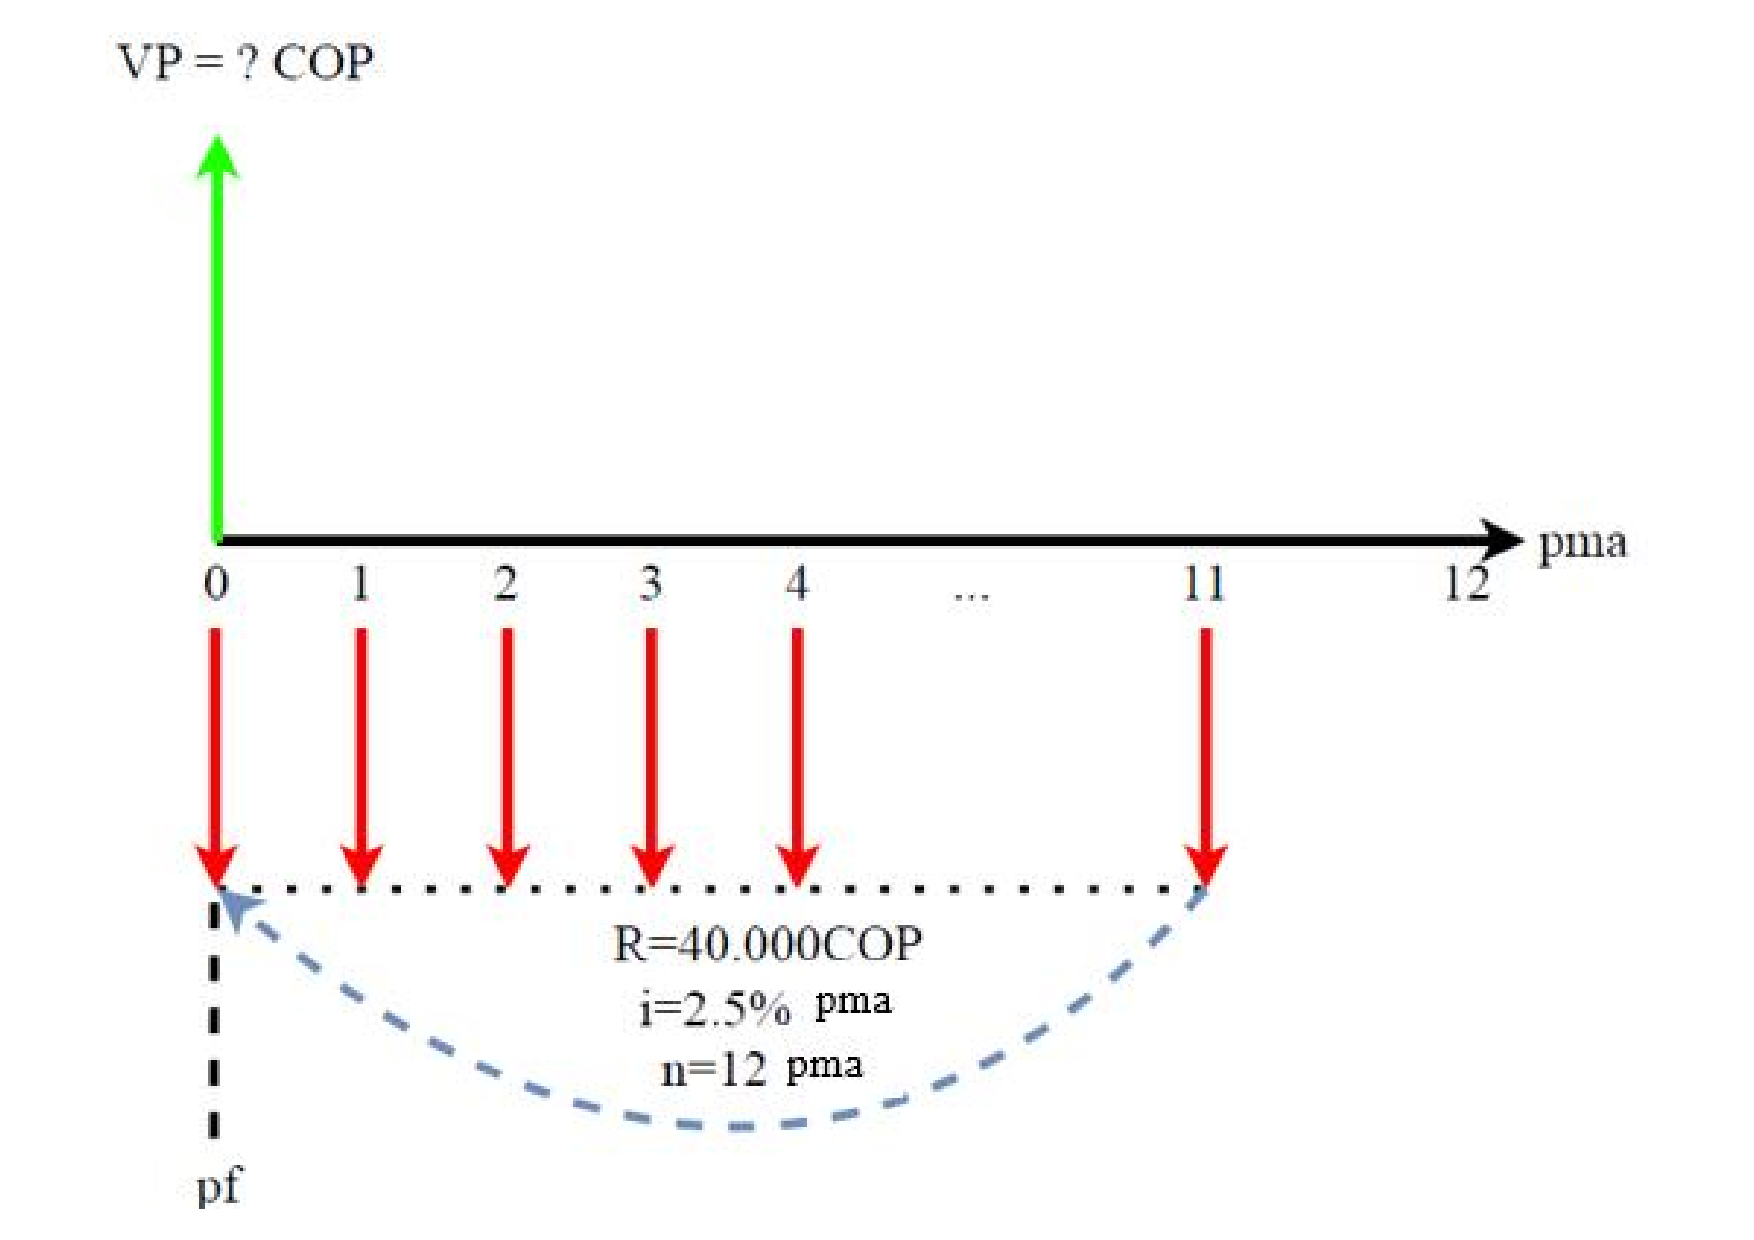
\includegraphics[width=0.90\columnwidth, trim=-5 -5 -5 -10]{4_Capitulo/img/ejemplos/6/Exportados/Ejemplo 5.pdf}  } \\ \hline
  %%%%%%%%%%%%% FIN INSERCIÓN DE IMAGEN
  %%%%%FIN FLUJO DE CAJA



  %%%%% INICIO DECLARACIÓN FORMULAS
  %%%%%%%%%%% INICIO TITULO
  \rowcolor[HTML]{FFB183}
  \multicolumn{3}{|c|}{\cellcolor[HTML]{FFB183}\textbf{4. Declaración de fórmulas}}                          \\ \hline
  %%%%%%%%%%% FIN TITULO
  %%%%%%%%%%% INICIO MATEMÁTICAS

  \multicolumn{3}{|c|}{{$VP_{a}=R \frac{1-(1+i)^{-n}}{i} (1+i)$} \hspace{0.3cm} {Valor presente serie uniforme anticipada}}    \\ \hline                                       
  \multicolumn{3}{|c|}{\cellcolor[HTML]{FFB183}\textbf{5. Desarrollo matemático}}                            \\ \hline
  %%%%%%%%%% FIN TITULO
  %%%%%%%%%% INICIO MATEMÁTICAS
  \multicolumn{3}{|c|}{ R = 840.000 \ $n = 12$\  $i=0.025$ \quad } \\
  \multicolumn{3}{|c|}{$VP_{a}=$40.000 COP$\frac{1-(1+0,025)^{-12}}{0,025}\textcolor{red}*(1+0,025)$  }     \\                  
  \multicolumn{3}{|c|}{ $VP_{a}=$420.568,35 COP  }  \\ \hline
  %%%%%%%%%% FIN MATEMÁTICAS
  %%%%%% FIN DESARROLLO MATEMÁTICO

  \rowcolor[HTML]{FFB183}
  \multicolumn{3}{|c|}{\cellcolor[HTML]{FFB183}\textbf{6. Respuesta}}                                        \\ \hline

  \multicolumn{3}{|c|}{El valor del pago unico será de 420.568 COP}                                                                \\ \hline
 \end{longtable}
 %Se crean dos lineas en blanco para que no quede el siguiente texto tan pegado
 %\newline \newline
\end{center}
%%%%%%%%%%%%%%%%%%%%%%%%%%FIN EJERCICIO 6 %%%%%%%%%%%%%%%%%%%%%%%%%%
%%%%%%%%%%%%%%%%%%%%%%%%%%FIN EJERCICIO 5%%%%%%%%%%%%%%%%%%%%%%%%%%%




	\section{Otro enfoque de las series periódicas anticipadas}
	Podemos calcular el valor presente de la serie uniforme anticipada como si fuera una serie uniforme vencida, de la siguiente manera, si retiramos el pago que está en 0 y también retiramos el período que se inicia en 11 y termina en 12, nos queda una serie ordinaria de 11 pagos con 11 períodos, luego forma una serie uniforme vencida porque empieza en período y termina con pago, el pago que está en cero se puede considerar como un pago adicional que no pertenece a la serie uniforme, tal como se aprecia en la gráfica anterior.\\

	Este enfoque es el más utilizado al resolver ejercicios de series periódicas anticipadas.
 %%%%%%%%%%%%%%%%%%% EJERCICIO 4 %%%%%%
%%%%%%%%%% NO OLVIDAR COLOCAR ESTE COMENTARIO CON EL NUMERO DE EJERCICIO %%%%%%%%%%%%%
%%%%%%%%%%%%%%%%%%% EJERCICIO 6 %%%%%%
%%Text bf para negrilla , el \\ es para el salto de linea.
%%El primer \\ hace un espacio en el texto y el 2 \\ crea otro espacio
\textbf{Traslado períodos anticipados a períodos vencidos}\newline
El siguiente diagrama representa un traslado de períodos anticipados a períodos vencidos, sin afectar la serie.\\ \\

\textbf{Solución.}\\
\begin{center}

 \renewcommand{\arraystretch}{1.5}% Margenes de las celdas
 %Creación de la cuadricula
 \begin{longtable}{|c|c|c| }
  %Creamos una linea horizontal
  \hline
  %Definimos el color de la primera fila
  \rowcolor[HTML]{FFB183}
  %%%%% INICIO ASIGNACIÓN FECHA FOCAL %%%%%%%
  %%%%%%%%%% INICIO TITULO
  %Lo que se hace aquí es mezclar las 3 columnas en una sola
  \multicolumn{3}{|c|}{\cellcolor[HTML]{FFB183}\textbf{1. Asignación período focal}}                           \\ \hline
  %%%%%%%%%% FIN TITULO
  %%%%% INICIO DECLARACIÓN DE VARIABLES %%%%%%%
  \multicolumn{3}{|c|}{$pf : 0 pma$}                                                                         \\ \hline
  %Definimos el color de la primera fila
  \rowcolor[HTML]{FFB183}
  %%%%% INICIO DECLARACIÓN DE VARIABLES %%%%%%%
  %%%%%%%%%% INICIO TITULO
  \multicolumn{3}{|c|}{\cellcolor[HTML]{FFB183}\textbf{2. Declaración de variables}}                         \\ \hline
  %%%%%%%%%% FIN TITULO
  %%%%%%%%%% INICIO DE MATEMÁTICAS
  \multicolumn{1}{|c|}{\cellcolor[HTML]{FFB183}\textbf{Valores monetarios}}    & \multicolumn{1}{c|}{\cellcolor[HTML]{FFB183}\textbf{Valores no monetarios}} & \multicolumn{1}{c|}{\cellcolor[HTML]{FFB183}\textbf{Incógnitas}} \\ \hline
  R= 40.000 COP & $i=2,5\% pmv$ & VP = ? COP\\
  $P_{0}=$ 40.000 COP & $n={11}\ pmv$ & \\
  & $n_{0}=12 pmv$ & \\ \hline

  %%%%%%%%%% FIN DE MATEMÁTICAS
  %%%%% FIN DECLARACIÓN DE VARIABLES


  %%%%% INICIO FLUJO DE CAJA
  \rowcolor[HTML]{FFB183}
  \multicolumn{3}{|c|}{\cellcolor[HTML]{FFB183}\textbf{3. Diagrama de flujo de caja}}                        \\ \hline
  %Mezclamos 3 columnas y pondremos el dibujo
  %%%%%%%%%%%%% INSERCIÓN DE LA IMAGEN
  \multicolumn{3}{|c|}{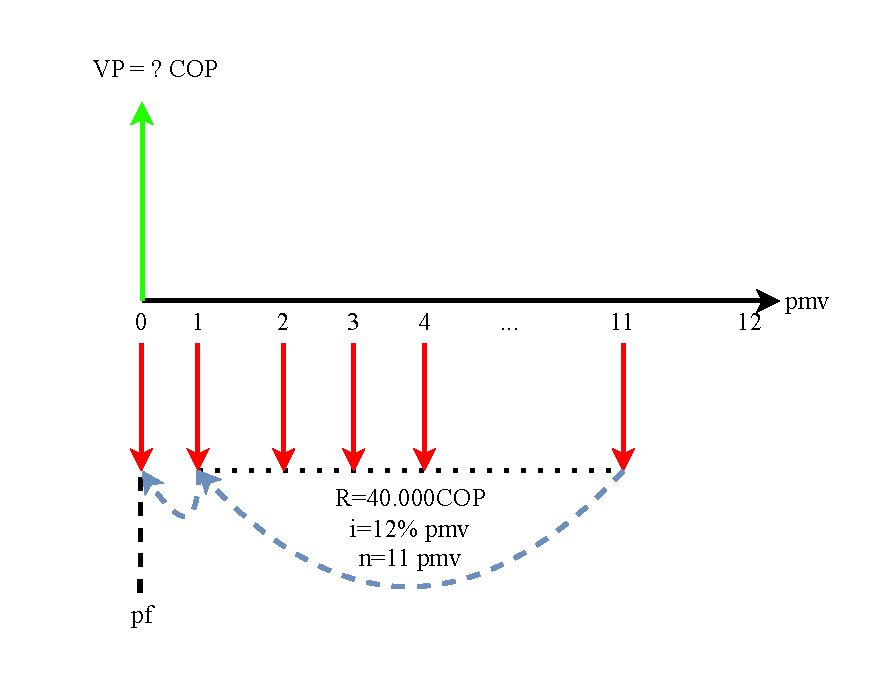
\includegraphics[width=0.95\columnwidth, trim=-3 -3 -3 -7]
  {4_Capitulo/img/ejemplos/Exportados/Ejemplo.pdf }} \\ \hline
  %%%%%%%%%%%%% FIN INSERCIÓN DE IMAGEN
  %%%%%FIN FLUJO DE CAJA



  %%%%% INICIO DECLARACIÓN FORMULAS
  %%%%%%%%%%% INICIO TITULO
  \rowcolor[HTML]{FFB183}
  \multicolumn{3}{|c|}{\cellcolor[HTML]{FFB183}\textbf{4. Declaración de fórmulas}}                          \\ \hline
  %%%%%%%%%%% FIN TITULO
  %%%%%%%%%%% INICIO MATEMÁTICAS
  \multicolumn{3}{|c|}{VP=R$\frac{(1-(1+i)^{-n})}{i}$ \hspace{35pt}{Valor presente serie uniforme vencida}}    \\ \hline                                       
  \multicolumn{3}{|c|}{\cellcolor[HTML]{FFB183}\textbf{5. Desarrollo matemático}}                            \\ \hline
  %%%%%%%%%% FIN TITULO
  %%%%%%%%%% INICIO MATEMÁTICAS
  \multicolumn{3}{|c|}{  $VP_{1}=$ 40.000 COP $\frac{1-(1+0,025)^{-11}}{0,025}$}\\
  \multicolumn{3}{|c|}{  $VP_{1}=$ 380.568,35 COP}\\
  \multicolumn{3}{|c|}{  $VP=VP_{1}+P_{0}$}\\
  \multicolumn{3}{|c|}{  $VP=$ 380.568,35 COP + 40.000 COP}\\ 
  \multicolumn{3}{|c|}{  $VP=$ COP 420.568,35 COP}\\ \hline
  %%%%%%%%%% FIN MATEMÁTICAS
  %%%%%% FIN DESARROLLO MATEMÁTICO

  \rowcolor[HTML]{FFB183}
  \multicolumn{3}{|c|}{\cellcolor[HTML]{FFB183}\textbf{6. Respuesta}}                                        \\ \hline

  \multicolumn{3}{|c|}{El valor del pago unico será de 420.568 COP}   \\ \hline
  
 \end{longtable}
 %Se crean dos lineas en blanco para que no quede el siguiente texto tan pegado
 %\newline \newline
\end{center}
%%%%%%%%%%%%%%%%%%%%%%%%%%FIN EJERCICIO 6 %%%%%%%%%%%%%%%%%%%%%%%%%%%
%%%%%%%%%%%%%%%%%%%%%%%%%%FIN EJERCICIO 4%%%%%%%%%%%%%%%%%%%%%%%%%%%
%%%%%%%%%%%%%%%%%%% EJERCICIO 6 %%%%%%
%%%%%%%%%% NO OLVIDAR COLOCAR ESTE COMENTARIO CON EL NUMERO DE EJERCICIO %%%%%%%%%%%%%
%%%%%%%%%%%%%%%%%%% EJERCICIO 7 %%%%%%
%%Text bf para negrilla , el \\ es para el salto de linea.
%%El primer \\ hace un espacio en el texto y el 2 \\ crea otro espacio
\textbf{Ejemplo 6}\newline
Una persona necesita tener reunidos 100.000 COP para el día 15-10-95, para tal fin constituye un fondo mediante depósitos trimestrales de R efectuándose el primero el día 15-7-90 y el último el 15-4-95 además se efectuará un depósito extraordinario de 8.000 COP el 15-1-93. Si el fondo paga el 24\% nominal anual trimestre vencido. ¿Cuál es el valor de la cuota de la serie uniforme? Considerar un año de 360 días.\\ \\

\textbf{Solución.}\\
\begin{center}

 \renewcommand{\arraystretch}{1.5}% Margenes de las celdas
 %Creación de la cuadricula
 \begin{longtable}{|c|c|c| }
  %Creamos una linea horizontal
  \hline
  %Definimos el color de la primera fila
  \rowcolor[HTML]{FFB183}
  %%%%% INICIO ASIGNACIÓN FECHA FOCAL %%%%%%%
  %%%%%%%%%% INICIO TITULO
  %Lo que se hace aquí es mezclar las 3 columnas en una sola
  \multicolumn{3}{|c|}{\cellcolor[HTML]{FFB183}\textbf{1. Asignación período focal}}                             \\ \hline
  %%%%%%%%%% FIN TITULO
  %%%%% INICIO DECLARACIÓN DE VARIABLES %%%%%%%
  \multicolumn{3}{|c|}{$pf : 0 ptv$}                                                                           \\ \hline
  %Definimos el color de la primera fila
  \rowcolor[HTML]{FFB183}
  %%%%% INICIO DECLARACIÓN DE VARIABLES %%%%%%%
  %%%%%%%%%% INICIO TITULO
  \multicolumn{3}{|c|}{\cellcolor[HTML]{FFB183}\textbf{2. Declaración de variables}}                           \\ \hline
  %%%%%%%%%% FIN TITULO
  %%%%%%%%%% INICIO DE MATEMÁTICAS
  \multicolumn{1}{|c|}{\cellcolor[HTML]{FFB183}\textbf{Valores monetarios}}    & \multicolumn{1}{c|}{\cellcolor[HTML]{FFB183}\textbf{Valores no monetarios}} & \multicolumn{1}{c|}{\cellcolor[HTML]{FFB183}\textbf{Incógnitas}} \\ \hline
  VF= 100.000 COP & $j=24\% natv\equiv 6\% ptv =i$ & R= ? COP \\
  P= 8.000 COP & $n_{1}=20$ ptv & \\
  & $n_{2}=2 $ ptv & \\ 
  & $n_{3}=11 $ ptv & \\ \hline

  %%%%%%%%%% FIN DE MATEMÁTICAS
  %%%%% FIN DECLARACIÓN DE VARIABLES


  %%%%% INICIO FLUJO DE CAJA
  \rowcolor[HTML]{FFB183}
  \multicolumn{3}{|c|}{\cellcolor[HTML]{FFB183}\textbf{3. Diagrama de flujo de caja}}                          \\ \hline
  %Mezclamos 3 columnas y pondremos el dibujo
  %%%%%%%%%%%%% INSERCIÓN DE LA IMAGEN
  \multicolumn{3}{|c|}{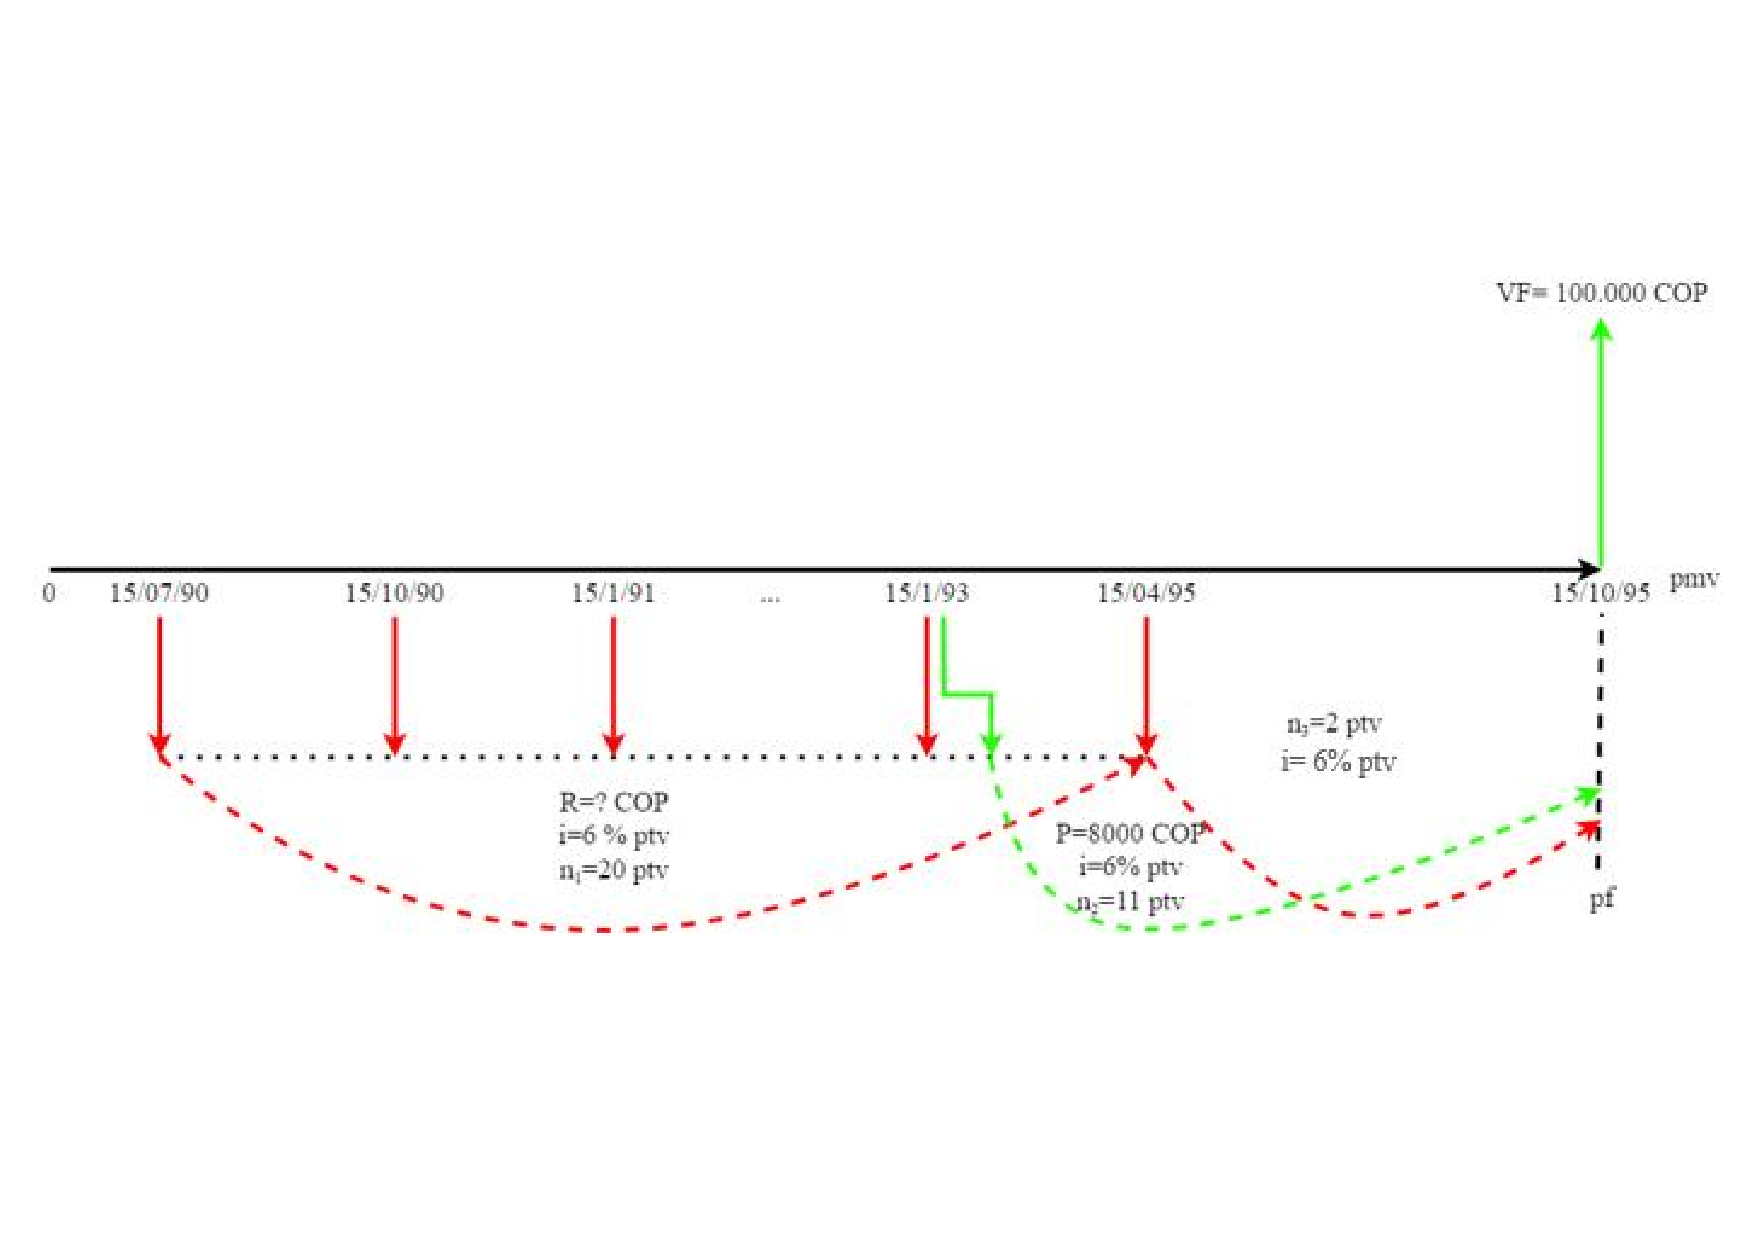
\includegraphics[width=0.95\columnwidth, trim=-5 -5 -5 -10]{4_Capitulo/img/ejemplos/7/Exportados/Ejemplo6.pdf}}   \\ \hline
  %%%%%%%%%%%%% FIN INSERCIÓN DE IMAGEN
  %%%%%FIN FLUJO DE CAJA



  %%%%% INICIO DECLARACIÓN FORMULAS
  %%%%%%%%%%% INICIO TITULO
  \rowcolor[HTML]{FFB183}
  \multicolumn{3}{|c|}{\cellcolor[HTML]{FFB183}\textbf{4. Declaración de fórmulas}}                            \\ \hline
  %%%%%%%%%%% FIN TITULO
  %%%%%%%%%%% INICIO MATEMÁTICAS

  \multicolumn{3}{|c|}{$VF = R \frac{((1+i)^{n}-1)}{i}$ Valor futuro serie uniforme vencida} \\ 
  \multicolumn{3}{|c|}{$F = P(1+i)^{n}$ Valor futuro}\\ \hline
  %%%%%%%%%% FIN MATEMÁTICAS
  %%%%%% INICIO DESARROLLO MATEMÁTICO
  \rowcolor[HTML]{FFB183}
  %%%%%%%%%%INICIO TITULO
  \multicolumn{3}{|c|}{\cellcolor[HTML]{FFB183}\textbf{5. Desarrollo matemático}}                              \\ \hline
  %%%%%%%%%% FIN TITULO
  %%%%%%%%%% INICIO MATEMÁTICAS
  \multicolumn{3}{|c|}{$R\frac{(1+0,06)^{20}-1}{0,06}\textcolor{red}*(1+0,06)^{2}+$ 8.000 COP $\textcolor{red}*(1+0,06)^{11}=$100.000 COP} \\ \hline
  %%%%%%%%%% FIN MATEMÁTICAS
  %%%%%% FIN DESARROLLO MATEMÁTICO

  \rowcolor[HTML]{FFB183}
  \multicolumn{3}{|c|}{\cellcolor[HTML]{FFB183}\textbf{6. Respuesta}}                                          \\ \hline

  \multicolumn{3}{|c|}{El valor de la cuota es de 2.051,99 COP}                                                                         \\ \hline
 \end{longtable} 
 %Se crean dos lineas en blanco para que no quede el siguiente texto tan pegado
\end{center}
%%%%%%%%%%%%%%%%%%%%%%%%%%FIN EJERCICIO X %%%%%%%%%%%%%%%%%%%%%%%%%%%

%%%%%%%%%%%%%%%%%%%%%%%%%%FIN EJERCICIO 6%%%%%%%%%%%%%%%%%%%%%%%%%%%
   


    \section{Amortización}

    La amortización de una obligación o deuda, se define como el proceso mediante el cual se paga la deuda junto con sus intereses, en una serie de pagos y en un tiempo determinado, se representa mediante la letra R.\\
    
    Cuando se adquiere una obligación, su pago se pacta con una serie de condiciones mínimas que determinan el comportamiento que debe asumir el deudor: valor de la deuda, plazo, tasa de interés y patrón de pago.\\


	\section{Tabla de amortización}
	La amortización consiste en pagar una deuda, mediante una serie de pagos; el comportamiento de la deuda y los intereses se pueden mostrar en una tabla denominada tabla de amortización.\\
	Una tabla de amortización debe tener como mínimo, cinco columnas: la primera muestra el número del período, la segunda nos muestra el saldo de la deuda, es decir, el capital insoluto a medida que van pasando los períodos, la tercera nos muestra los intereses que se van causando período a período, la cuarta columna nos muestra la cuota o cantidad que se paga en cada período y la quinta columna nos muestra la porción de la cuota que se usa para disminuir la deuda, es decir, la cantidad que se amortiza, también se le denomina abono a capital.
	\vspace{1mm}

	Haciendo uso del ejemplo 9 explicaremos la forma de construir una tabla de amortización.\\

 %%%%%%%%%%%%%%%%%%% EJERCICIO 7 %%%%%%

%%%%%%%%%% NO OLVIDAR COLOCAR ESTE COMENTARIO CON EL NUMERO DE EJERCICIO %%%%%%%%%%%%%
%%%%%%%%%%%%%%%%%%% EJERCICIO 9 %%%%%%
%%Text bf para negrilla , el \\ es para el salto de linea.
%%El primer \\ hace un espacio en el texto y el 2 \\ crea otro espacio
\textbf{Ejemplo 7}\newline
Elaborar una tabla para amortizar la suma de 10.000.000 COP en 4 pagos iguales, suponiendo una tasa de interés de 40\% nominal anual trimestre vencido.\\ \\

\textbf{Solución.}\\
\begin{center}

    \renewcommand{\arraystretch}{1.5}% Margenes de las celdas
    %Creación de la cuadricula
    \begin{longtable}{|c|c|c| }
        %Creamos una linea horizontal
        \hline
        %Definimos el color de la primera fila
        \rowcolor[HTML]{FFB183}
        %%%%% INICIO ASIGNACIÓN FECHA FOCAL %%%%%%%
        %%%%%%%%%% INICIO TITULO
        %Lo que se hace aquí es mezclar las 3 columnas en una sola
        \multicolumn{3}{|c|}{\cellcolor[HTML]{FFB183}\textbf{1. Asignación período focal}}   \\ \hline
        %%%%%%%%%% FIN TITULO
        %%%%% INICIO DECLARACIÓN DE VARIABLES %%%%%%%
        \multicolumn{3}{|c|}{$pf : 0 ptv$} \\ \hline
        %Definimos el color de la primera fila
        \rowcolor[HTML]{FFB183}
        %%%%% INICIO DECLARACIÓN DE VARIABLES %%%%%%%
        %%%%%%%%%% INICIO TITULO
        \multicolumn{3}{|c|}{\cellcolor[HTML]{FFB183}\textbf{2. Declaración de variables}}      \\ \hline
        %%%%%%%%%% FIN TITULO
        %%%%%%%%%% INICIO DE MATEMÁTICAS
        \multicolumn{1}{|c|}{\cellcolor[HTML]{FFB183}\textbf{Valores monetarios}}    & \multicolumn{1}{c|}{\cellcolor[HTML]{FFB183}\textbf{Valores no monetarios}} & \multicolumn{1}{c|}{\cellcolor[HTML]{FFB183}\textbf{Incógnitas}} \\ \hline
        $VP =$ 10.000.000 COP & $j=40\% natv \equiv 10\% ptv =i$ & $R= ? COP $ \\ 
        & $n=4$ ptv & \\ \hline

        %%%%%%%%%% FIN DE MATEMÁTICAS
        %%%%% FIN DECLARACIÓN DE VARIABLES


        %%%%% INICIO FLUJO DE CAJA
        \rowcolor[HTML]{FFB183}
        \multicolumn{3}{|c|}{\cellcolor[HTML]{FFB183}\textbf{3. Diagrama de flujo de caja}}         \\ \hline
        %Mezclamos 3 columnas y pondremos el dibujo
        %%%%%%%%%%%%% INSERCIÓN DE LA IMAGEN
        \multicolumn{3}{|c|}{ 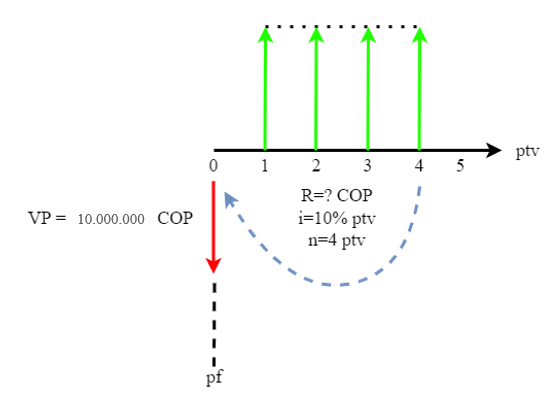
\includegraphics[scale=0.6, trim=-5 -5 -5 -5]{4_Capitulo/img/ejemplos/10/Exportados/Ejemplo7.png}  } \\ \hline 
        %%%%%%%%%%%%% FIN INSERCIÓN DE IMAGEN
        %%%%%FIN FLUJO DE CAJA



        %%%%% INICIO DECLARACIÓN FORMULAS
        %%%%%%%%%%% INICIO TITULO
        \rowcolor[HTML]{FFB183}
        \multicolumn{3}{|c|}{\cellcolor[HTML]{FFB183}\textbf{4. Declaración de fórmulas}}       \\ \hline
        %%%%%%%%%%% FIN TITULO
        %%%%%%%%%%% INICIO MATEMÁTICAS

        \multicolumn{3}{|c|}{$VP=R\frac{1-(1+i)^{-n}}{i}$ Valor presente serie uniforme vencida}  \\ \hline
        %%%%%%%%%% FIN MATEMÁTICAS
        %%%%%% INICIO DESARROLLO MATEMÁTICO
        \rowcolor[HTML]{FFB183}
        %%%%%%%%%%INICIO TITULO
        \multicolumn{3}{|c|}{\cellcolor[HTML]{FFB183}\textbf{5. Desarrollo matemático}}    \\ \hline
        %%%%%%%%%% FIN TITULO
        %%%%%%%%%% INICIO MATEMÁTICAS
        \multicolumn{3}{|c|}{10.000.000 COP$=R\frac{1-(1+0,1)^{-4}}{0,1}$ }     \\ \hline
        %%%%%%%%%% FIN MATEMÁTICAS
        %%%%%% FIN DESARROLLO MATEMÁTICO

        \rowcolor[HTML]{FFB183}
        \multicolumn{3}{|c|}{\cellcolor[HTML]{FFB183}\textbf{6. Respuesta}}    \\ \hline

        \multicolumn{3}{|c|}{R=3.154.708 COP} \\
        \multicolumn{3}{|c|}{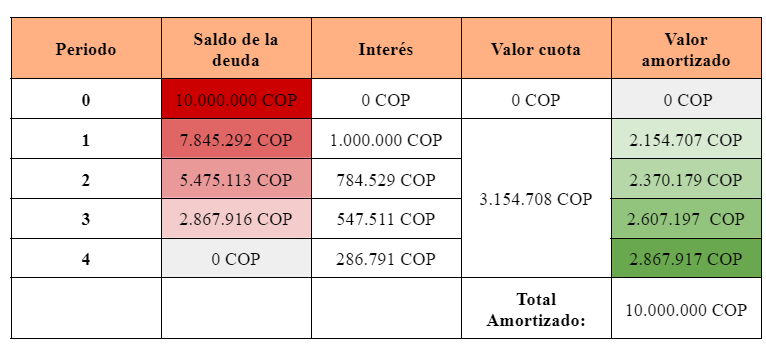
\includegraphics[scale=0.8, trim=-5 -5 -15 -15]{4_Capitulo/img/ejemplos/9/Exportados/Amortizacion.png}} \\ \hline  


    \end{longtable}
    %Se crean dos lineas en blanco para que no quede el siguiente texto tan pegado
    %\newline \newline
\end{center}
%%%%%%%%%%%%%%%%%%%%%%%%%%FIN EJERCICIO X %%%%%%%%%%%%%%%%%%%%%%%%%%%

%%%%%%%%%%%%%%%%%%%%%%%%%%FIN EJERCICIO 7%%%%%%%%%%%%%%%%%%%%%%%%%%%
   

	
        \section{Capitalización}
        La palabra capitalización tiene otros significados afines, en esta guía por capitalización entenderemos el reunir un capital mediante depósitos periódicos.
	\\\\
	\section{Tabla de capitalización}
	
	Una tabla de capitalización nos muestra, período a período, la forma como se va reuniendo un capital, su conformación es similar a la de amortización y básicamente debe tener 5 columnas que en su orden las denominaremos: período, capital reunido o monto, intereses, depósito o cuota y la última columna que se denomina capitalización o incremento por período.
	\\\\
	La explicación de la forma de elaborar una tabla de capitalización la daremos con el siguiente ejemplo:
	\\\\
 %%%%%%%%%%%%%%%%%%% EJERCICIO 8 %%%%%%

%%%%%%%%%% NO OLVIDAR COLOCAR ESTE COMENTARIO CON EL NUMERO DE EJERCICIO %%%%%%%%%%%%%
%%%%%%%%%%%%%%%%%%% EJERCICIO 10 %%%%%%
%%Text bf para negrilla , el \\ es para el salto de linea.
%%El primer \\ hace un espacio en el texto y el 2 \\ crea otro espacio
\textbf{Ejemplo 8}\newline
Elaborar una tabla para capitalizar la suma de 300.000 COP en 15 meses, haciendo depósitos trimestrales iguales en un fondo que paga una tasa del 32\% nominal anual trimestre vencido.\\ \\

\textbf{Solución.}\\
\begin{center}

	\renewcommand{\arraystretch}{1.5}% Margenes de las celdas
	%Creación de la cuadricula
	\begin{longtable}{|c|c|c| }
		%Creamos una linea horizontal
		\hline
		%Definimos el color de la primera fila
		\rowcolor[HTML]{FFB183}
		%%%%% INICIO ASIGNACIÓN FECHA FOCAL %%%%%%%
		%%%%%%%%%% INICIO TITULO
		%Lo que se hace aquí es mezclar las 3 columnas en una sola
		\multicolumn{3}{|c|}{\cellcolor[HTML]{FFB183}\textbf{1. Asignación período focal}}   \\ \hline
		%%%%%%%%%% FIN TITULO
		%%%%% INICIO DECLARACIÓN DE VARIABLES %%%%%%%
		\multicolumn{3}{|c|}{$pf : 5 ptv$} \\ \hline
		%Definimos el color de la primera fila
		\rowcolor[HTML]{FFB183}
		%%%%% INICIO DECLARACIÓN DE VARIABLES %%%%%%%
		%%%%%%%%%% INICIO TITULO
		\multicolumn{3}{|c|}{\cellcolor[HTML]{FFB183}\textbf{2. Declaración de variables}}      \\ \hline
		%%%%%%%%%% FIN TITULO
		%%%%%%%%%% INICIO DE MATEMÁTICAS
		\multicolumn{1}{|c|}{\cellcolor[HTML]{FFB183}\textbf{Valores monetarios}}    & \multicolumn{1}{c|}{\cellcolor[HTML]{FFB183}\textbf{Valores no monetarios}} & \multicolumn{1}{c|}{\cellcolor[HTML]{FFB183}\textbf{Incógnitas}} \\ \hline
		VF = 300.000 COP &	$j = 32\% \ natv \equiv  8\% ptv = i$ & $R= ? COP $\\ 
		& $n=5 \ ptv$ & \\ \hline

		%%%%%%%%%% FIN DE MATEMÁTICAS
		%%%%% FIN DECLARACIÓN DE VARIABLES


		%%%%% INICIO FLUJO DE CAJA
		\rowcolor[HTML]{FFB183}
		\multicolumn{3}{|c|}{\cellcolor[HTML]{FFB183}\textbf{3. Diagrama de flujo de caja}}         \\ \hline
		%Mezclamos 3 columnas y pondremos el dibujo
		%%%%%%%%%%%%% INSERCIÓN DE LA IMAGEN
		\multicolumn{3}{|c|}{ 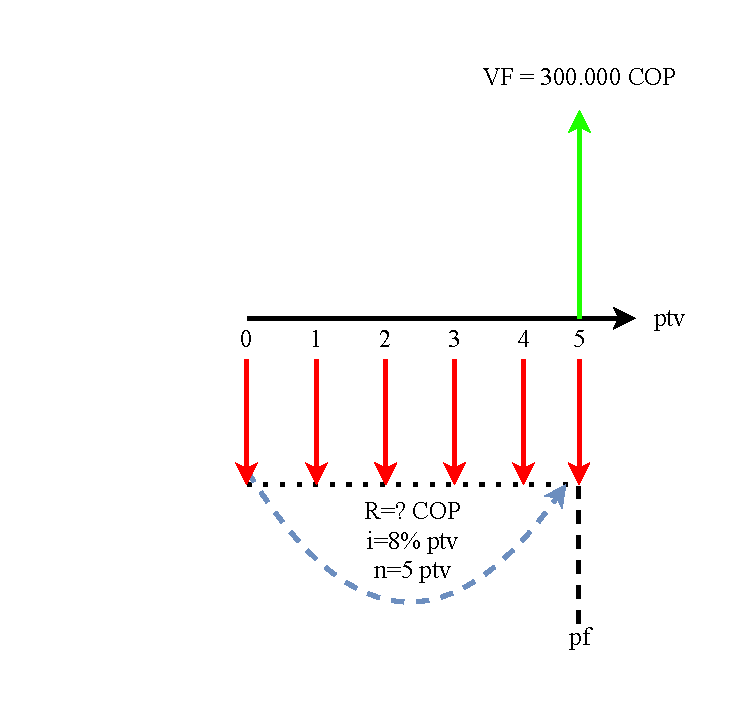
\includegraphics [scale=0.6, trim=-5 -5 -5 -5]{4_Capitulo/img/ejemplos/10/Exportados/Ejemplo 8.pdf}}     \\ \hline
		%%%%%%%%%%%%% FIN INSERCIÓN DE IMAGEN
		%%%%%FIN FLUJO DE CAJA



		%%%%% INICIO DECLARACIÓN FORMULAS
		%%%%%%%%%%% INICIO TITULO
		\rowcolor[HTML]{FFB183}
		\multicolumn{3}{|c|}{\cellcolor[HTML]{FFB183}\textbf{4. Declaración de fórmulas}}       \\ \hline
		%%%%%%%%%%% FIN TITULO
		%%%%%%%%%%% INICIO MATEMÁTICAS

		\multicolumn{3}{|c|}{$VF=R\frac{((1+i)^{n}-1)}{i}$ \hspace{35pt}{Valor futuro serie uniforme vencida}}   \\ \hline
		%%%%%%%%%% FIN MATEMÁTICAS
		%%%%%% INICIO DESARROLLO MATEMÁTICO
		\rowcolor[HTML]{FFB183}
		%%%%%%%%%%INICIO TITULO
		\multicolumn{3}{|c|}{\cellcolor[HTML]{FFB183}\textbf{5. Desarrollo matemático}}    \\ \hline
		%%%%%%%%%% FIN TITULO
		%%%%%%%%%% INICIO MATEMÁTICAS
		\multicolumn{3}{|c|}{300.000 COP $=R\frac{(1+0,08)^{5}-1}{0,08}$ }     \\ \hline
		%%%%%%%%%% FIN MATEMÁTICAS
		%%%%%% FIN DESARROLLO MATEMÁTICO

		\rowcolor[HTML]{FFB183}
		\multicolumn{3}{|c|}{\cellcolor[HTML]{FFB183}\textbf{6. Respuesta}}    \\ \hline

		\multicolumn{3}{|c|}{R= 51.136,9 COP} \\ \hline
		
		\multicolumn{3}{|c|}{  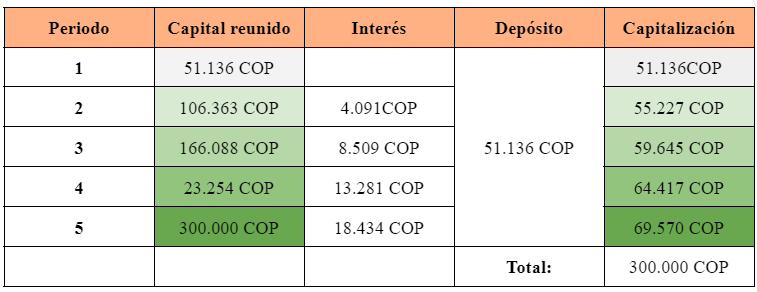
\includegraphics[scale=0.6, trim=-5 -5 -15 -15]{4_Capitulo/img/ejemplos/10/Exportados/Capitalizacion.png}} \\ \hline      
	\end{longtable}
	%Se crean dos lineas en blanco para que no quede el siguiente texto tan pegado
	%\newline \newline
\end{center}
%%%%%%%%%%%%%%%%%%%%%%%%%%FIN EJERCICIO X %%%%%%%%%%%%%%%%%%%%%%%%%%%

%%%%%%%%%%%%%%%%%%%%%%%%%%FIN EJERCICIO 8%%%%%%%%%%%%%%%%%%%%%%%%%%%
   
	


\clearpage
